\section{Signal- und Datenverarbeitung von Mess\-einrichtungen}

Datenerfassung oder auch Datenakquisition (\textit{engl. data acquisition}) wird häufig DAQ abgekürzt. In den folgenden Abschnitten wird die DAQ mittels
\begin{align*}
\mathrm{integrierter\,Messdatenerfassung\,}  &\textrm{via}\, \textbf{RS-232\,} \mathrm{Schnittstelle}, \\
\mathrm{analog\,Signalumwandlung\,mittels\,} \textbf{NI-USB\,6001\,} \mathrm{Messkarte\,} &\textrm{via}\, \textbf{USB\,}\mathrm{Schnittstelle}
\end{align*} 

unter der Verwendung von LabVIEW (2018, 2020 und 2021) erläutert. Für die Umsetzung wurden Anforderungen definiert, die wie folgt aufgelistet sind:

\begin{itemize}[leftmargin=*,labelsep=-\mylen]
\item Die Applikationen sollen eine graphische Oberfläche haben.
\item Der Aufwand für die Applikationsgenerierung soll minimal sein.
\item Die Applikationen sollen nur von ausgewählten Personal (\glqq leicht\grqq{}) anpassbar sein.
\item Die verwendete Software soll in der Lage sein, Daten der verschiedenste Versuchsstände und Geräte unterschiedlicher Hersteller abzubilden.
\item Es sollen Echtzeitgraphen generiert werden können.
\item Die verwendete Applikation soll kontinuierliche und diskrete Daten verarbeiten können.
\item Die Möglichkeit, die Daten in Zukunft direkt in eine Datenbank schreiben zu können, ist wünschenswert.
\end{itemize}


Es werden Module programmiert, mit denen kontinuierliche und diskrete Signalströme und Daten verarbeiten werden können. Somit ist es möglich, für alle Unit Operations Programme mittels LabVIEW zu schreiben. Diese diskreten Daten  können in einer separaten Datei oder als Header einer z.B. \,{\Menlo Tabulator} getrennten \glqq \,{\Menlo kontiMessungs.txt}\grqq{} Datei gespeichert werden. Man ist nicht daran gebunden als Spaltentrennzeichen (\textit{engl. delimiter}) \,{\Menlo Tabulator} zu verwenden, auch die Verwendung eines \,{\Menlo Komma} (\,{\Menlo *.csv} Datei), \,{\Menlo Semikolon} oder auch ein frei wählbares Trennzeichen ist möglich. Aufgrund der internationalen Konventionsunterschiede in Bezug auf das Dezimaltrennzeichen (ASCII \,{\Menlo '.'}, in Deutschland \,{\Menlo ','} etc.)  ist von der Verwendung eines \,{\Menlo Kommata} jedoch abzuraten.

\paragraph*{RS-232 zu USB Adapter} Wenn ein PC keine RS-232 Schnittstelle besitzt, kann ein RS-232 zu USB Adapter verwendet werden. Ein Mikroprozessor im Kabel emuliert eine RS-232 Schnittstelle. \\

\subsection{Serielle Schnittstellenkonfiguration und Signalverarbeitung von Messeinrichtungen}

In diesem Abschnitt werden virtuelle Instrumente (VI) zur Verarbeitung kontinuierlicher und diskreter Daten im ASCII Format (ASCII \,{\Menlo encoded}) programmiert, die über eine RS-232 Schnittstelle empfangen werden und die Daten verarbeitet. In der Abbildung \ref{fig:sensor_digitale_schnittstelle} ist zu erkennen, wie die hardwareseitige Datenverarbeitung im Falle eines Messgeräts mit integrierter digitaler Schnittstelle aussieht. Das Messobjekt, dass könnte bspw.. die gravimetrische Bestimmung eines Syntheseprodukts sein, wird messtechnisch mittels Sensor erfasst und transmittiert, dass im Messgerät bereits umgewandelte Signal, an einen Microcontroller (Arduino, RasPi ...), PC oder ähnliches.

\begin{figure}[h!] %[htbp!] 
\centering
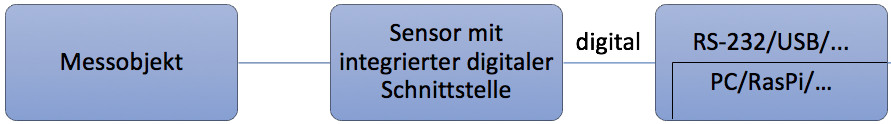
\includegraphics[width=0.9\textwidth]{Bilder/sensor_digitale_schnittstelle.jpg}
\vspace{0em}
 \caption[DAQ von Messeinrichtungen mit integrierter digitaler Schnittstelle]{DAQ von Messeinrichtungen mit integrierter digitaler Schnittstelle}\label{fig:sensor_digitale_schnittstelle}
\end{figure}

 Es werden die Schritte erklärt, wie man mit LabVIEW einen kontinuierlichen Datenstrom verarbeitet, der über eine RS-232 Schnittstelle empfangen wird. Es wird ein Windows 10 PC sowie ein Mac Book Pro und LabVIEW 2018 sowie LabVIEW 2020 verwendet, um die VI's zu programmieren und die Signale eines Messinstruments zu verarbeiten. Als Demonstrationsmesssystem wird eine Digitalwaage des Modells 440-47N des Herstellers KERN ausgelesen und die Daten interpretiert, die in eine Tabulator getrennten Text-Datei (\,{\Menlo *.txt}) geschrieben werden. Die Waage hat einen integrierten analog/digital Wandler und besitzt eine RS-232 Schnittstelle. Das Programm wird aus mehreren Sub VI's und dem Haupt VI bestehen. \\

%\begin{table}[h] % Serielle Konfigurationsparameter der Digitalwaage KERN 440-47N
%\caption{Sub VI's}
%\begin{center}
%\begin{tabular}{r|l}
%\onehalfspacing
%%\hline
%Serial Sub VI \hspace{6pt} & \hspace{6pt} Abbildung: \ref{step5} \\
%VTP Elapsed Time  \hspace{6pt} & \hspace{6pt} Abbildung: \ref{fig:vtp_elapsed_time}   \\
%Header Module \hspace{6pt} & \hspace{6pt} Abbildung: \ref{fig:modularer_header}  \\
%%\hspace{6pt} & \hspace{6pt}  \\
%
%%\hline
%\end{tabular}
%\end{center}
%\label{tab:subvis}
%\end{table}


\noindent In einem VI wird der Datenstrom, der von der Waage übermittelt wird, akquiriert. Das Sub VI wird folgend \,{\Menlo Serial Sub VI} oder in der Kurzform \textbf{\,{\Menlo SSVI}} genannt. Das \textbf{Haupt VI} wird die Daten, die es vom Sub VI erhält verarbeiten/interpretieren und in eine \,{\Menlo *.txt} Datei loggen. Des Weiteren soll das Haupt VI einen live plotter besitzen. Für einen modularen Header werden Sub VI's geschrieben, welcher Daten wie Gruppennummer, lokaler (des jeweiligen PC's) Datum- und Zeitstempel (modifizierbar), die VT Praktikums Nr. o.ä. enthält.\\

\noindent Um die korrekte Konfiguration Ihres Geräts vorzunehmen zu können, ist in dem Handbuch des Geräts nach folgenden Parametern zu schauen:

\begin{itemize} % RS-232 Parameter
\singlespacing
\item Zeichen Codierung, z.B. 7-\,{\Menlo Bit} 'ASCII'
\item \,{\Menlo Baudrate}
\item \,{\Menlo Paritätsbit}
\item \,{\Menlo Stopbit}
\item \,{\Menlo Flow Control}  (\textit{engl. dt. Flusssteuerung})
\end{itemize}

\noindent Die Digitalwaage sendet ihre digitalen Signale über eine RS-232 Schnittstelle, die 8-\,{\Menlo Bit} ASCII-encodiert sind. Um einen \textbf{kontinuierlichen Datenstrom} zu erhalten und somit \textbf{kontinuierlich} zu wiegen, wird in der Einstellung der Waage \glqq automatisches Senden\grqq{} eingestellt (das Gewicht soll gesendet werden, auch wenn der Wert nicht stabil ist). Die seriellen Konfigurationsparameter der Waage und des PC's bzw. des verarbeitenden Programms wie z.B. LabVIEW müssen identisch sein, um decodierbare Daten empfangen zu können. Diese Einstellungen sind über das Menü der Waage vorzunehmen. In der Tabelle \ref{tab:kern440} werden die verwendeten seriellen Konfigurationsparameter der Waage 440-47N des Herstellers Kern aufgelistet (Kurzschreibweise in  (\textit{engl. shorthand notation})).\\

\begin{table}[h] % Serielle Konfigurationsparameter der Digitalwaage Kern 440-47N
\caption{RS-232 Konfigurationsparameter der Digitalwaage Kern 440-47 N in shorthand \\ notation 8-N-1}
\begin{center}
\begin{tabular}{r|l}
\onehalfspacing
%\hline
\,{\Menlo Baudrate} in\,$\mathrm{s}^{-1}$ \hspace{6pt} & \hspace{6pt} \,{\Menlo 1200} \\
\,{\Menlo Byte}länge in \,{\Menlo Bit} \hspace{6pt} & \hspace{6pt} \textbf{\,{\Menlo 8}}  \\
\,{\Menlo Paritätsbit} \hspace{6pt} & \hspace{6pt} \,{\Menlo None (\textbf{N)}} \\
\,{\Menlo Stopbit} \hspace{6pt} & \hspace{6pt} \textbf{\,{\Menlo 1}} \\
\,{\Menlo Encoded} \hspace{6pt} & \hspace{6pt} ASCII \\
\,{\Menlo Flow-Control} \hspace{6pt} & \hspace{6pt} \,{\Menlo Software-Handshake} \\
%\hline
\end{tabular}
\end{center}
\label{tab:kern440}
\end{table}

\textbf{Anmerkung:} Für die Programmierung wurde eine Digitalwaage des Herstellers Kern des Typs 440-47 N gewählt. Das Programm wird auf andere Geräte übertragbar sein. Die einzige Anforderung ist, dass die RS-232 Parameter aufeinander abgestimmt werden.

\subsection{Serielle Schnittstelle im Betriebssystem finden und Debuggen} 

Die für den Benutzer sichtbare Benennung des RS-232 Ports unterscheidet sich zwischen den Betriebssystemen. Im Verlauf des Projekts wurde mit einem Unix (Mac Book Pro) und Windows 10 Betriebssystem gearbeitet. 

\paragraph*{Microsoft Windows} Bei der Verwendung eines Windows PC's wird der Port der seriellen Schnittstelle Com Port genannt und wird im Gerätemanager und in Programmen, wie z.B. in LabVIEW, \,{\Menlo COM 1-N} aufgelistet. 

\paragraph*{Mac Unix} Bei der Verwendung eines MACOS/Unix ist die serielle Schnittstelle im Terminal des Mac unter ~dev/tty.* und ~dev/cu.* zu finden und wird in LabVIEW \mbox{\,{\Menlo ASLR 1-N::INSTR}} genannt. \\

\noindent Um die richtigen Parameter zu identifizieren oder ob generell Signale, und wenn in welcher Form, empfangen werden kann mit einigen Tools ermittelt werden.

\paragraph{Tool zur Identifikation und Debuggen serieller Schnittstellen} Um herauszufinden ob die Konfigurationsparameter stimmen; ein Gerät Daten sendet, wie das Datenformat aussieht und ob die Daten korrekt übermittelt werden; kann man unter Windows das kostenlose Tool namens hTerm verwenden. Ein etwas weniger komfortables, jedoch vergleichbares open source Tool unter Mac oder Linux ist CoolTerm.\\

\subsection{Kontinuierliche Daten via RS-232 und LabVIEW verarbeiten}

Die grafische Programmiersprache G mit der Entwicklungsumgebung LabVIEW ist in der Lage Daten via RS-232 Schnittstelle zu akquirieren und zu interpretieren. Um eine serielle Schnittstelle in LabVIEW auslesen zu können, wird der \textbf{NI-VISA} Treiber benötigt. 

\footnotesize \singlespacing

 \noindent \textbf{Anmerkung:} Es werden unter MACOS einige Funktionen nicht unterstützt, wie unter anderem der LabVIEW Paketmanager und einige Pakete wie bspw. DAQmx für den Mac zu erhalten und zu implementieren hat \glqq Potentiall\grqq{}.

\normalsize \onehalfspacing


\subsubsection{Anpassung der LabVIEW-Einstellungen}
\label{sec:LabVIEW_Einstellungen}

Damit Texteingaben in Eingabefenstern (\textit{Control} Fenster) mit der Betätigung von Enter quittiert werden, ist in den LabVIEW Einstellungen folgender Haken zu setzen:

\begin{center}  % Tools > Options... > Category > Enviroment > End text entry ...
Tools > Options ... > Category > Enviroment > End text entry with Enter key [aktivieren]
\end{center} 

\noindent Wenn ein serieller Port geöffnet wird \textbf{ist es wichtig, dass bei dem Beenden des Programms der serielle Port geschlossen wird!} Wenn der Abbruch Button (\textit{engl. abort button}) von LabVIEW genutzt wird, wird der Port nicht geschlossen, daher soll das VI nur über den \textit{Stop Button} des Frontpanels geschlossen werden. Um den \textit{Abort Button} für das gerade verwendete VI (Programm) zu entfernen, gehen Sie bitte wie folgt vor:

\begin{center} % File > VI properties... > Window Apperance > Customize ...
File > VI properties > Window Apperance > Customize ... >  Show Abort button [deaktivieren]
\end{center} 

\input{Benötigte_LabVIEW_Objekte}
 
\subsubsection{Serielle Sub VI programmierung}

Zu Beginn wird ein VI oder wie auch nachfolgend \textit{Objekt} genannt programmiert (in LabVIEW auf englisch \textit{Function}). Dieses VI wird im folge Abschnitt in das Haupt VI als Sub VI mit dem Namen \textit{Serial Sub VI} integriert. Zu Beginn öffnet man ein neues leeres VI. Das \textit{Serial Sub VI}, im folgenden \textit{SSVI}, wird für die Konfiguration einer seriellen Schnittstelle verwendet. Die von LabVIEW verwendeten \textit{Objekte} können Sie den Tabellen \ref{tab:labviewserialobject} und \ref{tab:labviewserialobject2} entnehmen. In den Tabellen \ref{tab:labviewserialobject} und \ref{tab:labviewserialobject2} (die sich ebenfalls im Anhang befinden), sind alle Objekte aufgelistet die benötigt werden, um die \textit{VI's} zu programmieren. In den Tabellen \ref{tab:labviewserialobject} und \ref{tab:labviewserialobject2} wird das Blockdiagramm mit \textbf{BD}, das Front Panel mit \textbf{FP} und die rechte Maustaste mit \textbf{rM} abgekürzt. In den folgenden Programmierabbildungen sind die Funktion wie in den Tabellen \ref{tab:labviewserialobject} und \ref{tab:labviewserialobject2} nummeriert.\\

\paragraph{Erster Schritt: Serielle Objekte} Nach dem Erstellen eines neuen VI's fügt man alle Objekte ein, die man für den Datentransfer mit serieller Schnittstelle benötigt (4 - 9 in Tabelle \ref{tab:labviewserialobject}) (siehe Abbildung \ref{step1}). 

\bildp{h!}{1}
{LabVIEW_serialport/step_1_all_serial_functions_2.png}
{0em}
{Einfügen aller seriellen Funktionen}
{Einfügen aller seriellen Funktionen}
{step1}


\paragraph{Zweiter Schritt: Port Initialisierungs- und Abbruchskonfiguration} An dem Objekt \,{\Menlo Configure Port} sind Konstanten mit den Konfigurationswerten hinzuzufügen. An den Objekteingängen auf der linken Seite des Objekts, erstellt man Konstanten (rechte Maustaste/\,{\Menlo Create Constant} (11), siehe Abbildung \ref{step2}), die die seriellen Konfigurationsparameter enthalten (siehe Tabelle \ref{tab:kern440}). Um den Anwender dieses VI's den gesamten Kombinationsraum der Parameter zu Verfügung zu stellen, ist es auch möglich anstelle der Konstanten, \,{\Menlo Controls} zu verwenden. Anschließend zieht man eine \,{\Menlo Case-Structur} (2a) um das \,{\Menlo Configure Port} (zzgl. Konstanten) sowie das \,{\Menlo Flush Buffer} (9) Objekt und eine weitere \,{\Menlo Case-Structur} (2b) um das \,{\Menlo Close Port} Objekt. Wird die \,{\Menlo Case-Structure} (29) mittels eines Wahrheitswerts (\textit{boolean variable}, \,{\Menlo true}/\,{\Menlo false}) getriggert, wird somit der Port Konfiguriert und der I/O Buffer \textit{geflushed}. Die \,{\Menlo Case Structure} (2b), auf der rechten Seite wird mittels eines \,{\Menlo Stop Buttons} auf \,{\Menlo true} gestellt, um den Port mittels des \,{\Menlo Close} (8) Objekts zu schließen.\\

\noindent Den Stop \textit{Button} (14), die \textit{VISA ressource name} (13) zur Auswahl des Ports und den String \textit{Indicator} (12) (siehe Tabelle \ref{tab:labviewserialobject}, 12 - 14) fügt man z.B. über das Front Panel hinzu und positioniert die dazugehörigen Objekte, die automatisch im Blockdiagramm erscheinen, an der richtigen Positionen. Der \textit{Stop Button} wird mit dem \textit{Case Selektor} der zweiten \textit{Case-Structure} (2b) verbunden. Wird das Programm durch diesen \textit{Stop Button} beendet, wird somit der Port geschlossen. \textbf{Aufgrund dessen ist es wichtig, den VI Abbruch Button zu Deaktivieren: \emph{File > VI properties... > Window Apperance > Customize ... > [Markierung entfernen] Show Abort button}}. Ein \textit{Indicator} zum Anzeigen und zum weiterreichen des, durch das \textit{Read} Objekt (6) ausgelesenen Strings, wird an das \textit{Read} Objekt (6) angeschlossen. Die erste \textit{Case Structure} (2a) wird durch ein \textit{First Call?} (3) Objekt getriggert.\\

\begin{figure}[hp!]
\subfloat
	[Einfügen von Stop Button, Indicators und VISA resource]
	[Einfügen von Stop Button, Indicators und VISA resource \label{step2}]{
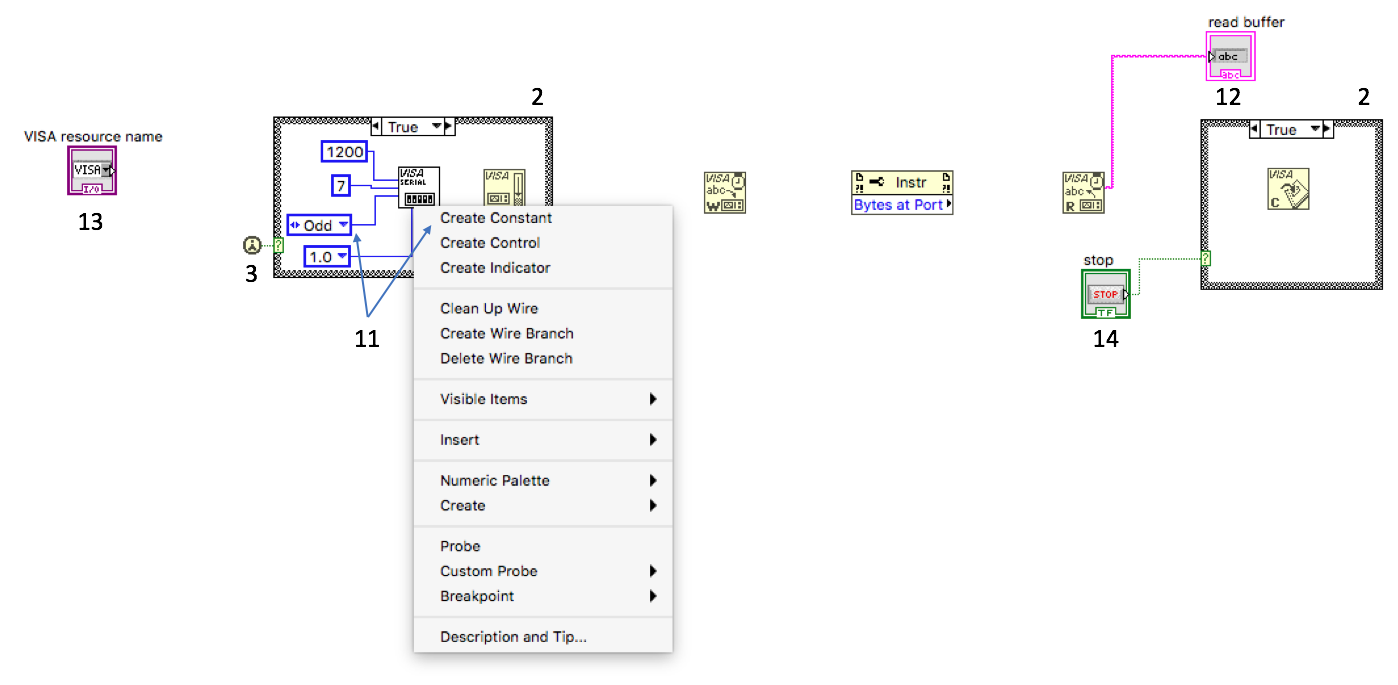
\includegraphics[width=1\textwidth]
	{Bilder/LabVIEW_serialport/step_2_cases_buttons-indicators-controls_2.png}
}
\phantomcaption
\vspace{5pt}
\ContinuedFloat
\subfloat
	[Einfügen von For Loop und Schieberegister]
	[Einfügen von For Loop und Schieberegister\label{step3}]{
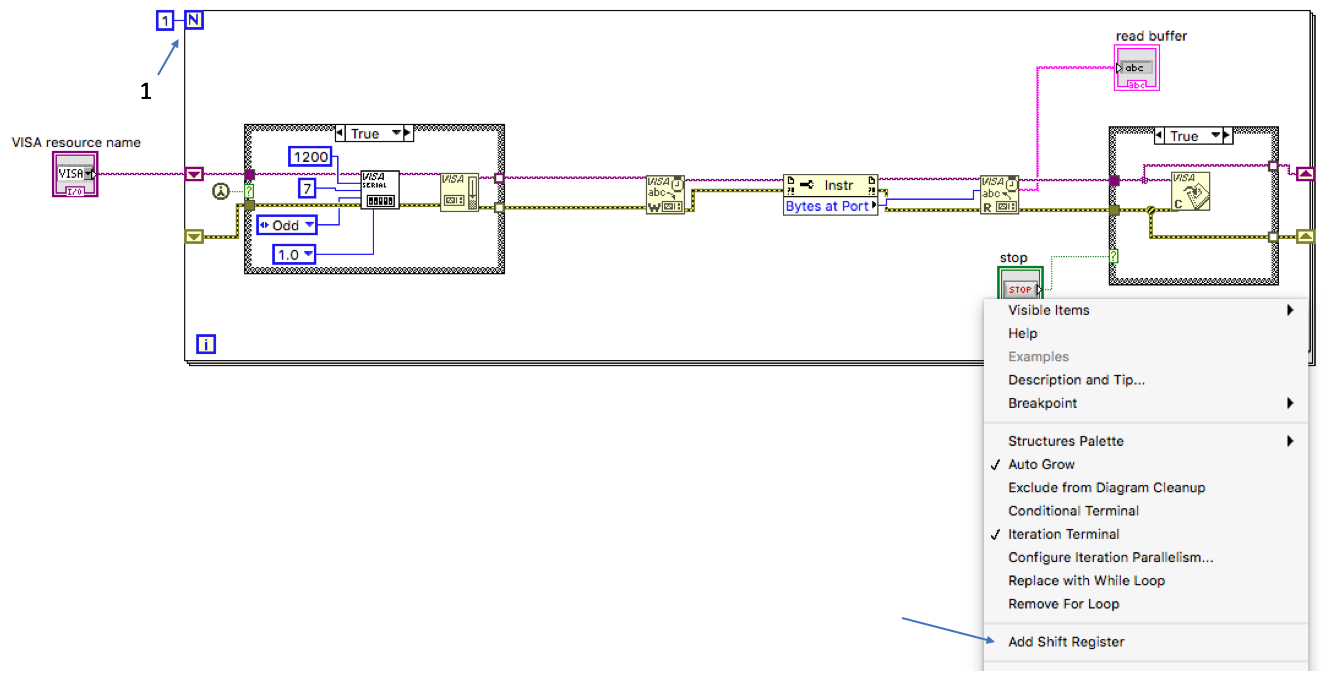
\includegraphics[width=1\textwidth]
	{Bilder/LabVIEW_serialport/step_3_for-loop_add-shift-register_2.png}
} 
\caption[]{Einfügen von Stop Button, Indicators, VISA resource, For Loops und Schieberegister}
\label{fig:step2_step3}
\end{figure}


\paragraph{Dritter Schritt: N = 1 For Loop, XON flow control}

Nun zieht man ein eine \,{\Menlo For} \,{\Menlo Loop} um alle Objekte, bis auf die \,{\Menlo VISA} \,{\Menlo Resource} und das \,{\Menlo Flush Buffer} Objekt. Die {\,{\Menlo For} \,{\Menlo Loop} wird in diesem Fall mit der Konstante 1 initialisiert (siehe Abbildung \ref{step3}, oben links). Nach dem hinzufügen von zwei Schieberegistern (\textit{engl. Shift Register}), sind alle Objekte wie in Abbildung \ref{step3} zu verdrahten. Durch das Hinzufügen eines \,{\Menlo Shift Registers} an einem Ende einer \,{\Menlo For Loop} oder \,{\Menlo While Loop}, werden automatisch die \,{\Menlo Shift Register} auf der anderen Seite des Loops generiert. Alle Funktionen müssen nun, wie in Abbildung \ref{step3}, verbunden werden (die blaue Leitung zwischen \,{\Menlo Bytes at Port} und \,{\Menlo Read Port} ist ebenfalls zu verbinden). Da die \glqq Verkabelung\grqq{} im \,{\Menlo true} Case beider \,{\Menlo Case Structures} verkabelt sind, muss selbiges noch im \,{\Menlo false} Case beider \,{\Menlo Case Structures} (2ab) geschehen (siehe Abbildung \ref{step3b}). Das \,{\Menlo Write} Objekt (7) ist mit der String Konstante (10) mit dem Wert \,{\Menlo 11} zu verknüpfen. Die \,{\Menlo String Konstante} \,{\Menlo 11} beinhaltet das ASCII flow control (siehe Abschnitt RS-232) Signal XON und signalisiert der Waage, dass der PC bereit ist Daten zu empfangen, da die Waage als \,{\Menlo flow control} den Software-Handshake verwendet. Technisch wird an die Waage der Hexadezimale \textit{character} 11 geschickt, also \,{\Menlo 0x11}. \,{\Menlo 0x11} ist das ASCII Hexadezimalzeichen für XON.  Dieses Objekt in dieser Form ist nun alleinstehend fähig den seriellen Port zu konfigurieren, der Waage das \,{\Menlo flow control} Signal XON zu senden, die Bytes auszulesen und darzustellen oder dem Haupt VI zu übergeben sowie den seriellen Port zu schließen, wenn das Programm über den Stop Button beendet wird.

\begin{figure}[h!p]
	\hfill     
     \subfloat[\glqq Verdrahtung\grqq{} der \,{\Menlo false} Cases]
     [\glqq Verdrahtung\grqq{} der \texttt{false} Cases\label{step3b}]{%
       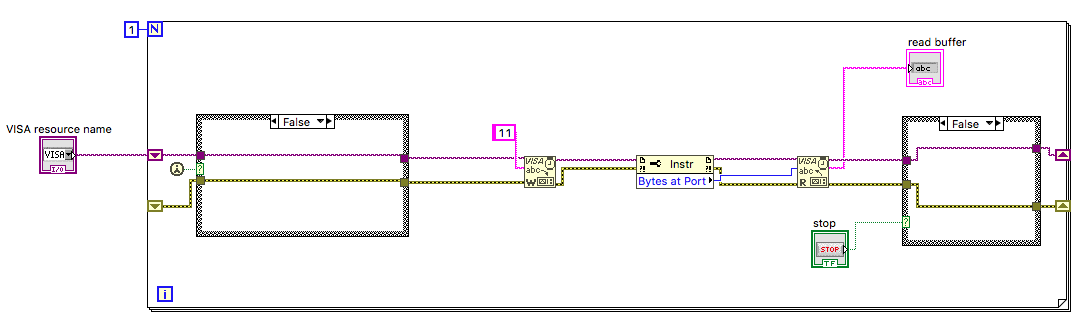
\includegraphics[width=0.99\textwidth]
       {Bilder/LabVIEW_serialport/step_3b_false_cases.png}
     }
     \phantomcaption
     \vspace{3pt}
\ContinuedFloat  
     \subfloat[Einfügen von For Loop und Schieberegister]
     [Optimiertes SSVI\label{step5}]{%
       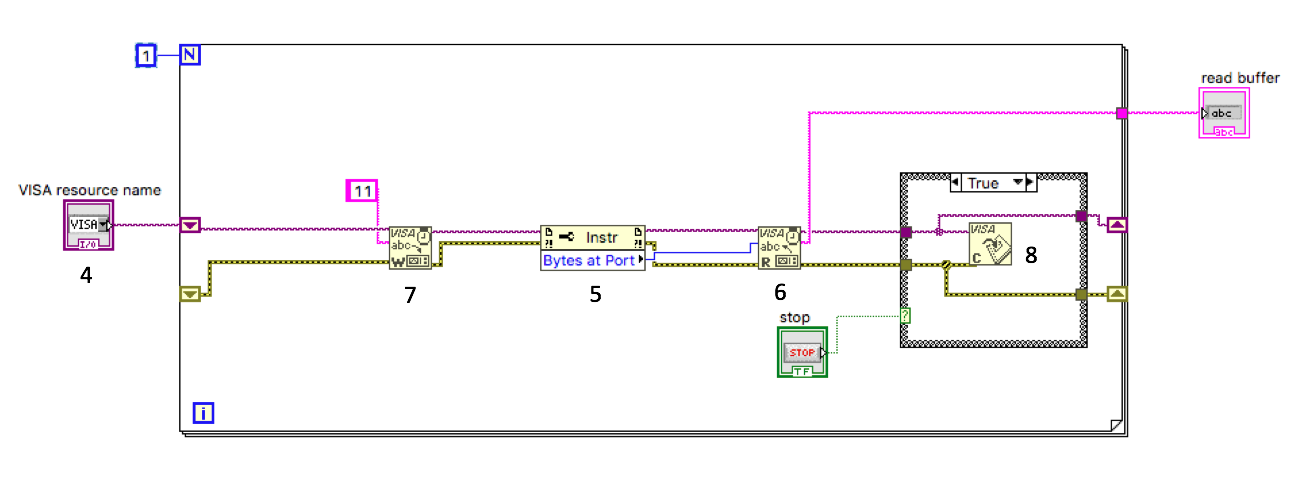
\includegraphics[width=1\textwidth]
       {Bilder/LabVIEW_serialport/step5_optimierung.png}
     }
     \caption[]{\glqq Verdrahtung\grqq{} der \,{\Menlo false} Cases und Optimiertes SSVI
  }
  \label{fig:step3b_step5}
\end{figure} % Einfügen von Stop Button, Indicators, VISA resource, For Loops und Schieberegister



\paragraph{Vierter Schritt: Optimierung} Das Programm in Abbildung \ref{step3} und \ref{step3b} konfiguriert bei jeder Iteration den Port und öffnet ihn. Das öffnen eines seriellen Ports, der bereits geöffnet ist, kann zu Störungen führen, daher sollte die Konfiguration des Ports über das Haupt-VI erfolgen. Der I/O-Buffer soll auch nur bei der ersten Iteration des Hauptprogramms gelöscht werden, der wird ebenfalls ins Haupt VI verlagert. In Abbildung \ref{step5} ist das Objekt nach der Optimierung abgebildet. Um den ausglesenen String nach Abschluss der Iteration an das Haupt VI übergeben zu können, wird der read Buffer rechts aus der For Loop geleitet. Das Objekt \,{\Menlo Configure Port} hat für den Inputbuffer per default 4096 \,{\Menlo Bytes} (Anmerkung: Sollte Ein I/O Buffer overflow o.ä. auftreten, dann könnte die Pause zwischen Iterationen zu lang sein). Mit Abschluss dieser Schritte ist das VI Objekt einsatzbereit und kann in mehrere Programmen, implementiert werden. Dafür müssen in der oberen rechten Ecke des Frontpanels die Ein- und Ausgänge des VI festgelegt werden (siehe Abbildung \ref{step4}, Nr. 16). Dazu klickt man auf ein Feld des Icons in der oberen rechten Ecke und auf eine Funktion, die sich im Frontpanel befindet. In diesem Beispiel wurde die obere rechte Ecke des mini Icons angewählt und mit einem Klick auf \,{\Menlo read buffer}, dem ausgelesenen String zugeordnet. Die obere linke Ecke des mini Icons wird mit VISA resource name und die Ecke unten links mit dem \,{\Menlo Stop Button} belegt.

\bild{.4}
{LabVIEW_serialport/step_4_VI_generieren_3.png}
{0em}
{Definition der VI Objekt Ein- und Ausgänge}
{Definition der VI Objekt Ein- und Ausgänge}
{step4}


\subsubsection{Kontinuierliche Messdatenerfassung RS-232 im Haupt VI}

Die Daten, die man via RS-232 empfängt, müssen interpretiert und in einer *.txt Datei gelogged werden. Die empfangenen Daten hängen von der verwendeten Messtechnik ab. Das Untersuchungsobjekt im Rahmen dieses Abschnitts ist eine Digitalwaage (KERN 440-47N). Das Datenformat dieser Waage ist wie folgt:

\begin{enumerate}
\singlespacing
\item Es können beliebig viele Leerzeichen zu Beginn des Strings vorhanden sein (\,{\Menlo '\textbackslash s'})
\item Es kann die Vorzeichen \,{\Menlo +} oder \,{\Menlo -} enthalten
\item Es können beliebig viele \,{\Menlo '\textbackslash s'} folgen
\item Es können beliebig viele Ziffern folgen
\item Es wird ein dezimal Trennungszeichen folgen (ASCII encodiert wäre es der Punkt \,{\Menlo '.'})
\item Es können wieder unbekannt viele Ziffern folgen
\item Es können beliebig viele \,{\Menlo '\textbackslash s'} folgen
\item Es kann die Maßeinheit \,{\Menlo 'g'} folgen, wenn der Messwert stabil ist
\item Es können beliebig viele \,{\Menlo '\textbackslash s'} folgen
\item Das Zeilenende kann je nach System variieren. Es kann \,{\Menlo '\textbackslash r'}, \,{\Menlo '\textbackslash n'}, \,{\Menlo '\textbackslash r''\textbackslash n'} oder \,{\Menlo '\textbackslash r\textbackslash n'} sein
\end{enumerate}


\paragraph{Erster Schritt: Port Konfiguration und String verketten/anzeigen lassen} Nach dem Erstellen eines neuen, leeren VI's, wird das VI des vorherigen Abschnitts per drag and drop in das leere VI gezogen. Dazu zieht man das Symbol 16 des \textit{SSVI} (siehe Abbildung \ref{step4}) in das neue VI. Als nächstes setzt man eine While Loop um dieses VI Objekt und verknüpft einen Stop Button (14) mit dem Stop Eingang des SSVI sowie dem Abbruchkriterium der While Loop (20). Außerhalb des Loops wird die Portkonfiguration (siehe Tabelle \ref{tab:kern440}) und das Objekt, welches den I/O Buffer (9) löscht, platziert. Um die Daten der Waage in Form eines Strings aus dem SSVI auszulesen, wird die Funktion zum Verketten von Strings \textit{engl. Concatenate Strings} (17) in den Loop platziert. Man benötigt Schieberegister (\textit{engl. Shift Register}), erweitert das \,{\Menlo Concatenate Strings} (17) Objekt auf zwei Eingänge und verbindet die \,{\Menlo Shift Register} mit der \textit{Concatenate Strings} (17) Funktion (links oberer Eingang des \textit{Concatenate Strings} (17) Objekts). Damit das \,{\Menlo Shift Register} bei der ersten Iteration (Index = 0, da LabVIEW, wie viele andere Programmiersprachen, 0 indexiert arbeitet) leer ist, wird das linke \,{\Menlo Shift Register} mit einer leeren String konstante gelöscht. In Abbildung \ref{step6} sind die beschriebenen Funktionen abgebildet. Um zu sehen ob und was empfangen und verkettet wird, fügen wir einen \,{\Menlo String Indicator} (21) ein. Da der Nutzer des Programms \,{\Menlo VISA Ressource} und \,{\Menlo String Indicator} sehen wird, ist es empfehlenswert es im FP in etwas eindeutiges umzubenennen. Um eindeutig erkennen zu können, welche Zeichen empfangen werden, kann man im Front Panel per rechts-klick in das entsprechende Fenster, die \,{\Menlo String Indicator} Anzeige in \,{\Menlo '\textbackslash'} umstellen (siehe Abbildung \ref{step6b}).

\bildp{h!}{0.7}
{LabVIEW_serialport/step6.png}
{0em}
{BD Haupt VI: SSVI Integration/Port Konfiguration/String\-operationen}
{BD Haupt VI: SSVI Integration, Port Konfiguration, String auslesen und \mbox{verketten}}
{step6}



\bild{0.4}
{LabVIEW_serialport/step6b.png}
{0em}
{FP Haupt VI: SSVI Integration/Port Konfiguration/String\-operationen}
{FP Haupt VI: SSVI Integration, Port Konfiguration, String auslesen und \mbox{verketten}}
{step6b}

\paragraph{Zweiter Schritt: \glqq String Slicing\grqq} Das VI verkettet den String bis zum Beenden des Programms. Um eine einzige abgeschlossene Zeichenkette (von String Beginn bis \,{\Menlo '\textbackslash n'}) zu erhalten, müssen wir den String kürzen (\textit{engl. slicing}). Dazu wird eine \,{\Menlo Case Structure} (2c) programmiert, die den String verkettet, bis die \,{\Menlo Search/Split String} (23) Funktion das von uns gesuchte Zeichen, das ASCII Steuerzeichen \,{\Menlo '\textbackslash n'} liest. Es können zwei Zustände vorliegen, \,{\Menlo true} und \,{\Menlo false}. 

\begin{quote}
Anmerkung: Bei der Funktion \,{\Menlo Configure Port} (4) ist per default \textit{Termination Character} auf \,{\Menlo true} gesetzt, was dazu führt, dass \,{\Menlo Read} (6) des SSVI beim decodieren der bytes, die sich im Input Buffer des Serial Ports befinden, beim decodieren des Steuerzeichens  \,{\Menlo '\textbackslash n'}, die Zeichenkette terminiert und alle weiteren Bytes, die sich im Input Buffer befinden, in der nächsten Iteration bis maximal zu einem \,{\Menlo '\textbackslash n'} gelesen und decodiert werden.
\end{quote}


\paragraph*{false} Die \,{\Menlo Search/Split String} Funktion soll nach einem \,{\Menlo '\textbackslash n'} Suchen. Der \textit{offset of match} Ausgang der Funktion gibt den Index des Matches im String an. Wenn die \,{\Menlo Search/Split String} Funktion das zu suchende Zeichen (in dieser Situation \,{\Menlo  '\textbackslash n'}) nicht findet, gibt \textit{offset of match} -1 wieder. Diese Information wird genutzt, um den \textit{Case Selektor} auf \texttt{false} zu setzen. 

Wenn der String kein \,{\Menlo '\textbackslash n'} enthält, gibt die Funktion als \,{\Menlo offset of match} den Index -1 zurück, demnach ist das boolsche Signal \texttt{true} aus der \,{\Menlo Equal?} (26) Funktion. Dieses Signal wird mit dem boolschen Operator \,{\Menlo Not} (27) negiert. Der \,{\Menlo Case Selector} (24) ist somit auf \,{\Menlo false} gesetzt.\\
Ist der \,{\Menlo Case Selector} (24) auf \,{\Menlo false}, wird der Draht, der den verketteten String (\,{\Menlo Shift Register} und \,{\Menlo SSVI}) enthält, in die \,{\Menlo Case Structure} (2c) geleitet und mit dem rechten \,{\Menlo Shift Register} verbunden.\newline

\noindent An dieser Stelle (siehe Abbildung \ref{slicing_bedingung}) wird nun eine \textbf{Sicherheit} eingebaut. Der String soll erst interpretiert werden, wenn die Länge des Strings größer einer Vorgabe ist. Die Länge einer Zeile kann dem Handbuch des jeweiligen Geräts entnommen werden oder sie wird durch das manuelle \textit{Debugging} z.B. hTerm oder trial and error eruiert. 


\begin{figure}[h!] 
\centering
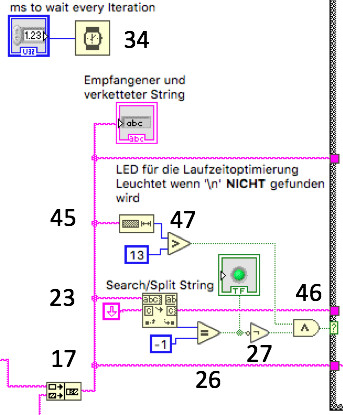
\includegraphics[width=0.4\textwidth]{Bilder/LabVIEW_serialport/slicing_bedingung.jpg}
\vspace{2pt}
\caption[Slicing Bedingung]{Slicing Bedingung}\label{slicing_bedingung}
\end{figure}

\paragraph*{true} Wenn der String \,{\Menlo '\textbackslash n'} enthält, gibt \textit{offset of match} dem \,{\Menlo Search/Split String} (23) Objekt den Index an, wo das Zeichen (in diesem Fall \texttt{'\textbackslash n'}) im String gefunden wurde. Der ist ungleich -1, der boolsche Zustand ist somit \,{\Menlo false} und wird mit der \,{\Menlo Not} (27) Funktion wieder in ein \,{\Menlo true} umgewandelt. Der \,{\Menlo Case Structure Selector} (24) ist damit auf \,{\Menlo true} gesetzt. Nun soll der Folgeiteration der Teil des Strings ab dem gesuchten Zeichen übergeben werden. Das kann mithilfe des Objekts \,{\Menlo String Subset} erreicht werden, indem man den Rest des Strings, des Objekts \,{\Menlo Search/Split String} (23), im \,{\Menlo true} Case, dem Objekt \,{\Menlo String Subset} (25) übergibt. Das Objekt \,{\Menlo String Subset} (25) wird die Konstante 1 der Funktion \textit{offset} zugewiesen. Durch diese Konfiguration der Funktionen wird der Rest des Strings \textbf{nach} dem gesuchten Zeichen (\,{\Menlo '\textbackslash n'}) dem \,{\Menlo Shift Register} (19) übergeben. Ist der PC und das Programm schneller als die empfangenen Daten, dann ist der übergebene String leer.

% \bild{1}
%{LabVIEW_serialport/step7_stringslicing.jpg}
%{-1em}
%{\glqq String Slicing\grqq{}: Dateninterpretation}
%{\glqq String Slicing\grqq{}: Dateninterpretation}
%{step7}

\begin{sidewaysfigure}
    \centering
    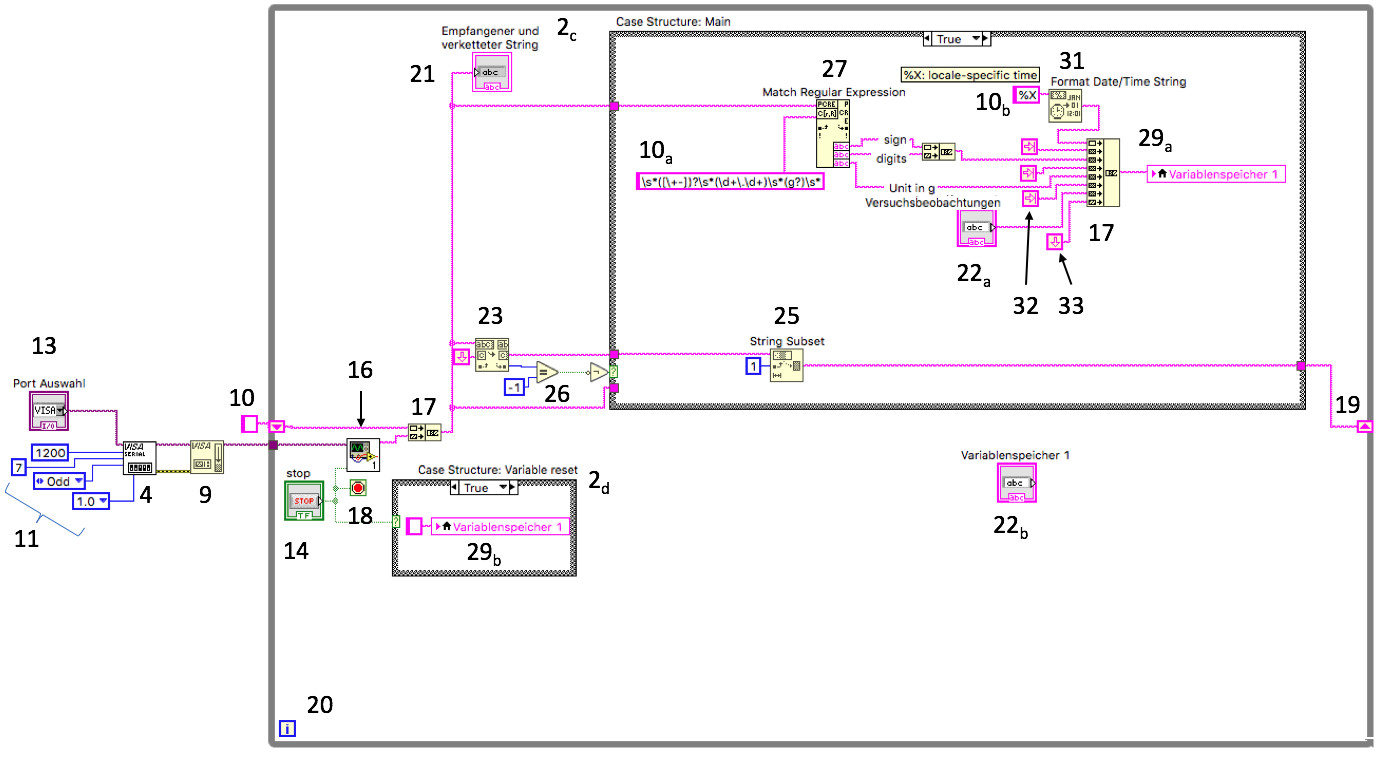
\includegraphics[width=1.04\textwidth]{Bilder/LabVIEW_serialport/step7_stringslicing.jpg}
    \caption[\glqq String Slicing\grqq{}: Dateninterpretation]{\glqq String Slicing\grqq{}: Dateninterpretation}
    \label{step7}
\end{sidewaysfigure}

\paragraph{Dritter Schritt: \glqq Dateninterpretation\grqq{}} Sobald eine vollständige Zeichenkette gelesen wurde, müssen die Daten in ihre Bestandteile zerlegt werden (siehe Abbildung \ref{step7}). In der \,{\Menlo Case Structure} (2c) wird im \,{\Menlo true}\, Case mit dem Objekt \,{\Menlo Regular Expression Match} (28), aus dem gesamten vorgelegten String alle gewünschten und potentiell vorkommenden Ausdrücke (\textit{engl. expressions}) separat extrahieren. In der folgenden Liste sind die Ausdrücke (\textit{engl. Submatches}) aufgelistet, die der String enthält, bzw. enthalten könnte.

\newpage 

\begin{itemize} % Submatch Expression
\singlespacing
\item Es kann ein \,{\Menlo '+'} oder \,{\Menlo '-'} enthalten
\item Beliebig viele \,{\Menlo '\textbackslash s'} (Leerzeichen)
\item Beliebig viele Ziffern
\item Dezimaltrennzeichen (unter ASCII \,{\Menlo '.'})
\item Beliebig viele Ziffern
\item Beliebig viele \,{\Menlo '\textbackslash s'}
\item Es kann ein \,{\Menlo 'g'} enthalten sein
\item Beliebig viele \,{\Menlo '\textbackslash s'}
\end{itemize}


 In der folgenden Liste werden die verwendeten \textit{Regular Expression} Operatoren erklärt.

\begin{itemize} %Submatch Expression Operatoren
\singlespacing
\item \texttt{(}x\texttt{)} generiert ein Submatch des Ausdrucks x
\item x\texttt{?} der Ausdruck x kann null oder einmal vorkommen
\item x\texttt{*} der Ausdruck x kann null oder viele male vorkommen
\item \texttt{\textbackslash d+} es können beliebig viele Ziffern (\textit{engl. digits}) vorkommen
\item \texttt{[}...\texttt{]} erstellt eine Zeichenklasse, die Angabe von \texttt{[}xyz\texttt{]} bedeutet, es kann x, y oder z vorkommen
	\begin{itemize} 
		\item[\small $\circ$] sollen Elemente der Zeichenklasse mehrfach vorkommen dürfen, dann ist \texttt{[}...\texttt{]} ein \texttt{+} nachzustellen, daraus folgt \texttt{[}xyz\texttt{]+} 
\end{itemize}
\end{itemize}

\noindent Dem Objekt \textit{Regular Expression Match} müssen wir folgenden Ausdruck in einer String Konstanten mitteilen, die drei Submatches generiert.

\begin{center} %Submatch Expressions
\texttt{
\textbackslash s*([\textbackslash +-])?\textbackslash s*(\textbackslash d+\textbackslash .\textbackslash d+)\textbackslash s*(g?)\textbackslash s*
}
\end{center}

\begin{description}  % Submatches
\singlespacing
\item[Submatch 1] ([\textbackslash +-)?
\item[Submatch 2] (\textbackslash d+\textbackslash .\textbackslash d+)
\item[Submatch 3] (g?)
\end{description}

\noindent Nun ist eine Stringzeile zu konstruieren (siehe Abbildung \ref{step7}). Das Ziel ist eine *.txt Datei, bei der die Spalten durch das \,{\Menlo Tabulator} Steuerzeichen (\,{\Menlo '\textbackslash t'}) (32) getrennt werden. \textbf{Beim Import einer, mit diesem Programm generierten, \,{\Menlo Ta\-bu\-lator-getrennt.txt}-Datei in, z.B. ein Tabellenkalkulationsprogramm, wie Excel, ist als Spaltentrennzeichen Tabulator anzugeben.} Für die Konstruktion (Verkettung von Strings) einer Zeile verwendet man das \,{\Menlo Concatenate} (17) Objekt. Ein String wird in einer textbasierten Programmiersprache wie Python mit Anführungsstrichen (\,{\Menlo ''}) deklariert. Das Objekt \textit{Concatenate} verkettet Strings.

\begin{center}
\textit{Concatenate} (17) bewirkt folgendes: \mbox{(\mbox{'ich bin'} + \mbox{'ein String'} = \mbox{'ich bin ein String'})}
\end{center}  

\noindent LabVIEW's \,{\Menlo Read} (6) Objekt liest \,{\Menlo Bit}-seriell vom Port, versendet nach dem Lesen \,{\Menlo Byte} seriell. Eine von der Waage gesendete Zeile könnte wie folgt aussehen:

\begin{figure}[h!] %Waagen String vor LabVIEW
\centering
\begin{BVerbatim}
'\s''\+''\s''\s''\s''\s''12''\.''8''\s''g''\s''\r''\n'
\end{BVerbatim}
\end{figure}


\noindent Bei dem \,{\Menlo Configure Port} Objekt (4) ist per default\textit{ Termination Character} auf\, \,{\Menlo true} gesetzt, d.h. \,{\Menlo Read} (6) liest bis zu einem\, \,{\Menlo '\textbackslash n'}. Der Rest verbleibt für die folgenden Iterationen im Input Buffer. Eine vollständig von \,{\Menlo Read} (6) gelesene Zeile ergibt somit folgenden String:


\begin{figure}[h!] %Waagenstring nach LabVIEW
\centering
\begin{varwidth}{\linewidth}
\begin{verbatim}
'\s\+\s\s\s\s12\.8\sg\s\r\n'
\end{verbatim}
\end{varwidth}
\end{figure}


\noindent Nun sollen die drei potentiellen Bestandteile (\texttt{ '+' }, \texttt{ '12.8' }, \texttt{ 'g' }) extrahiert werden. Das Vorzeichen und der Character \,{\Menlo 'g'} können, müssen aber nicht vorkommen. Die drei Submatches sind somit: 
\vspace{-2pt}
\begin{center}  \texttt{ '+' },\texttt{ '12.8' },\texttt{ 'g' } \end{center}

\noindent Mit den drei Elementen soll eine Datalogger Zeile generiert werden. Die Zeile soll wie folgt aufgebaut sein.

\begin{figure}[h!] %Spaltenformatierung
\begin{center}
\begin{varwidth}{\linewidth}
\begin{verbatim}
  Zeitstempel \t Messwert \t Einheit in g \t Versuchsbeobachtung \n
\end{verbatim}
\end{varwidth}
\end{center}
\end{figure}

\paragraph{Vierter Schritt: Zeilenkonstruktion} Das Programm wird Zeile für Zeile den Inhalt, der in die Tabgetrennte.txt Datei geschrieben werden soll, vorerst als String verketten. Dieser String wird nach dem Stoppen des Programms in die *.txt Datei geschrieben. Für die Konstruktion einer String Zeile wird das \textit{Concatenate} (17) Objekt genutzt (siehe Abbildung \ref{fig:String-/Zeilenkonstruktion}). Eine Dataloggerzeile wird in dieser Konfiguration (17, 22a, 31, 10b, 32, 33 und 29a), wie im vorherigen Abschnitt gefordert, konstruiert. Die Versuchsbeobachtungen werden mittels \textit{Control} (22a) dem jeweiligen Zeitstempel zugeordnet. Nach dem Schreiben in die *.txt Datei muss die \textit{Control} (22a) mit einem leeren String gelöscht werden (siehe Abschnitt \ref{sec:Datalogger} Abbildung \ref{datalogger}). Die verkettete Zeile ist einem \textit{Control} mittels einer lokalen Variable dem \textit{Variablenspeicher 1} (29a) zu übermitteln. Mit der Information, die im \textit{Variablenspeicher 1} hinterlegt wird, ist das kontinuierliche Loggen in eine *.txt, mit \,{\Menlo '\textbackslash t'} als delimiter möglich.

\begin{figure}[h!] % String-/Zeilenkonstruktion
	\centering
	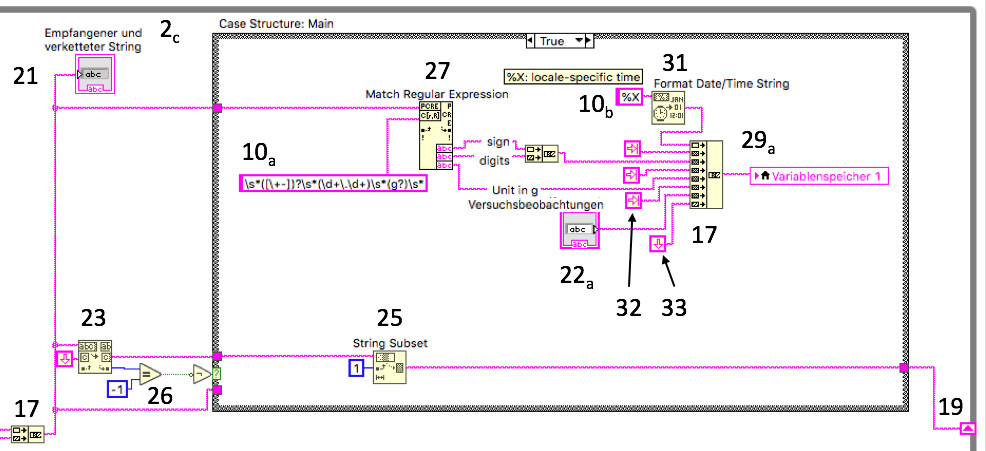
\includegraphics[width=1.05\textwidth]{Bilder/LabVIEW_serialport/stringkonstruktion.jpg}
	\vspace{2pt}
	\caption[String-/Zeilenkonstruktion]{String-/Zeilenkonstruktion}
	\label{fig:String-/Zeilenkonstruktion}
\end{figure}


\paragraph{Fünfter Schritt: Zeitstempelprogrammierung}  Der Zeitstempel (\textit{engl. Time\-stamp}) kann durch die folgenden zwei Methoden implementiert werden. Bei der ersten Methode wird mittels des Objekts \textit{Format Date/Time String} (siehe Abbildung \ref{fig:String-/Zeilenkonstruktion} (31) und (10b)) eine frei formatierbare Zeitreihe möglich (für genauere Infos schauen Sie bitte in \cite{zeitreihenformatierung}). \\

\noindent Um als Zeitstempel die verstrichene Zeit in ms zu bekommen, ist das Objekt wie in der Abbildung \ref{fig:vtp_elapsed_time} zu Programmieren (VTP Elapsed Time Sub VI) (44). Durch diese Methode ist es möglich bei Aktivierung dieses VI`s eine Startzeit zu ermitteln. Die Startzeit wird für den Header und für den Start des Datalogs, nach Betätigung der Start {\Menlo Datalogging in Tabgetrennt.txt} Datei, benötigt. Aus diesem Grund sind zwei Kopien dieses VI`s nötig!

%%=================================================================================

\input{Benötigte_LabVIEW_Konfigurationsfunktionen_Teil_2}

%%=================================================================================
 

\begin{figure}[!ht] %Methode 2   simple Elapsed Time in ms Sub VI (37)
     \subfloat[][\texttt{true}\label{fig:true}]
     {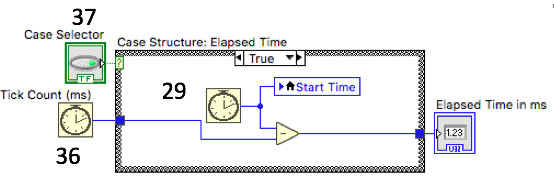
\includegraphics[width=0.5\textwidth]
       {Bilder/LabVIEW_serialport/step7_elapsed_true.jpg}
     }
     \hfill     
     \subfloat[][\texttt{false}\label{fig:false}]
     {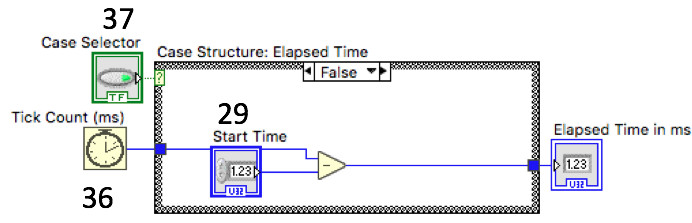
\includegraphics[width=0.5\textwidth]
       {Bilder/LabVIEW_serialport/step7_elapsed_false.jpg}
     }
     \caption[]{Methode 2 \glqq VTP Elapsed Time in ms\grqq{} Sub VI (37)\\     	
  }
  \label{fig:vtp_elapsed_time}
   \end{figure}


\paragraph{Sechster Schritt: Versuchsbeobachtungen} Es ist eine Kommentarfunktion gewünscht. Das Kommentar soll eingegeben werden können und nach der Bestätigung der Eingabe mit\, \,{\Menlo Enter}, soll der Kommentar zum Zeitpunkt der\, \,{\Menlo Enter} betätigung dem jeweiligen Zeitstempel zugeordnet werden. Dafür ist die Einstellung gemäß Abschnitt \ref{sec:LabVIEW_Einstellungen} vorzunehmen. Ein \textit{\textbf{Control}} Objekt (22) kann als Variablenspeicher interpretiert werden. Nach der Übergabe eines Wertes an das \,{\Menlo Control} Objekt des Kommentar muss diese nach der Ausgabe wieder gewiped werden. Zum \glqq löschen\grqq{} der letzten Eingabe in \,{\Menlo Control} Objekten, ist diese mit einer leeren Stringkonstanten zu überschreiben (siehe Abbildung \ref{datalogger} ) 29a. Der Programmablauf wäre dann wie folgt:


\begin{itemize} % Versuchsbeobachtungsreset
\singlespacing
\item Versuchsbeobachtung wird eingegeben (22a)
\item \textit{Case Selektor} wird getriggert durch Programmstart oder wenn die Dauer für ein Messwertaufnahmeintervall verstrichen ist
\item sobald der Datalogger Case Selektor getriggert wird, schaltet die \,{\Menlo Case Structure} auf \,{\Menlo true}
\item Löschen der \textit{Control Versuchsbeobachtung} durch die lokale Variable (298) 
\end{itemize}


\paragraph{Siebter Schritt: Dataloggerprogrammierung}
\label{sec:Datalogger}

Die Messwerte sollen in eine \,{\Menlo Tabulator} getrennte *.txt geschrieben werden. Als nächstes ist ein Datalogger zu programmieren (siehe Abbildung \ref{datalogger}). Mit den Objekten 38 bis 42 kann ein Datalogger programmiert werden, der jede \,{\Menlo While Loop} Iteration die Daten in ein *.txt schreibt, die er in der jeweiligen Iteration übergeben bekommt. Während einer Iteration, kann er beliebig viele Zeilen in die *.txt Datei schreiben. Im \,{\Menlo true} Case wird der String aus \textit{Variablenspeicher 1} in die *.txt Datei geschrieben, die in 40b, vor Programmausführung zu benennen ist (\,{\Menlo test\_aller\_Funktionen\_Beispiel.txt}). Mit dem \,{\Menlo Elapsed Time} Objekt (35) kann ein \,{\Menlo Control} Objekt programmiert werden, mit dem das Wertaufnahmeintervall in s eingestellt werden kann. Diese wird mit der Funktion \,{\Menlo Time Target} (s)} des \,{\Menlo Elapsed Time} (43) Objekts verbunden. Über diese Control kann man das Messwertaufnahmeintervall varieren, auch während des Programmablaufs. Der \textit{Time has Elapsed} boolsche Ausgang ist mit einem \,{\Menlo Or} (46) zu verbinden \,{\Menlo Case Selector}. Wenn der Iterations Index 0 oder die angegebene Zeit verstrichen ist, wird ein Messwert gelogged, bzw. alle Zeile in die *.txt Datei geschrieben, die dem \textit{Write to Text File} (38) Objekt übergeben wird. Im \,{\Menlo false} Case soll nix passieren, daher werden die Tunnel (insgesamt 2 x 2) beider \,{\Menlo Case Structure} Seiten mit einander verbunden. Der \textit{Variablenspeicher 1} wird mit einem leeren String gelöscht (\textit{engl. wiped}, umgangsprachlich gewiped). Damit ist der \textit{Variablenspeicher 1} bis zur nächsten Eingabe geleert.

\bild{1.05}
{LabVIEW_serialport/step8_datalogger.jpg}
{-1em}
{Datalogger}
{Datalogger}
{datalogger}

\paragraph{Siebter Schritt ergänzung gemäß neuster Applikationen: Graph mit zwei Plots}


Anmerkung: Aus zeitlichen Gründen wird auf eine genaue Bezeichnung verzichtet. Die Initialisierung gemäß Abbildung \ref{datalogger} ist zu erweitern, damit der Datalog per Knopfdruck geschehen kann. Die \textit{case structure} hat eine {\Menlo and} Bedingung erhalten, damit das Datalogging per Knopfdruck getriggert wird (siehe Abbildung \ref{fig:datalogger_inie_true}). In Abbildung \ref{fig:datalogger_inie_true} und \ref{fig:datalogger_inie_false} ist das {\Menlo VTP\_ElapsedTime.vi} zu erkennen. Damit bekommt der Datalogger eine Startzeit. In der Abbildung \ref{fig:Graphfürzwei} ist die Erstellung des Graphen mit zu erkennen. Der Graph ist zum Plotten der Arrays {\Menlo Volumenstrommesswerte\_arr\_input} und {\Menlo Druckmesswerte\_arr\_input}. Die Arrays werden mit der Build Array Methode pro Iteration erweitert. Damit im Verlauf der Messung auch Zahlen im Blockdiagramm erkennbar sind wurde jeweils ein {\Menlo Array Indicator} dem Draht hinzugefügt und die Anzeige gespiegelt. Die Spiegel dient dazu, dass der neuste Wert oben im Array angezeigt wird. Der Graph bekommt seine Zeitreihenwerte vom {\Menlo VTP\_ElapsedTime2.vi} (siehe Abbildung \ref{fig:datalogger_inie_true}). Die Zeitreihen und Messwert Arrays werden mittels {\Menlo Cluster Bundle} zusammengeführt. Die erstellten {\Menlo Cluster} werden mittel der {\Menlo Build Array Methode} zusammengeführt und dem Graph als Dateninput geliefert. Das Graph VI kann aus einem Build XY Graph extrahiert werden (Doppelklick \> Strg +E etc.). Für den {\Menlo false case} werden alle Drähte mit dem zugehörigen {\Menlo shift register} verbunden.

\begin{figure}[p!] % 
% \captionsetup{position=top}
    \centering
        \subfloat[][Graph/Dataloggerinitialiserung true \label{fig:datalogger_inie_true}]{%
            \hspace{0em}
            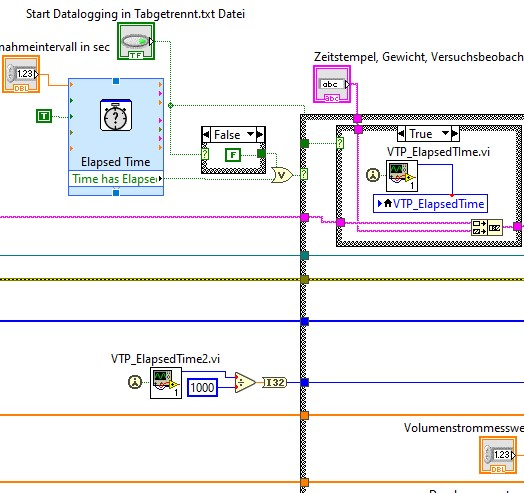
\includegraphics[width=0.55\textwidth]
            {Bilder/LabVIEW_serialport/datalogger_links_neu.jpg} %{Bilder/LabVIEW_serialport/}
        }\hspace{0.05em}
        \subfloat[][Graph/Dataloggerinitialiserung false \label{fig:datalogger_inie_false}]{%
            \hspace{0em}
            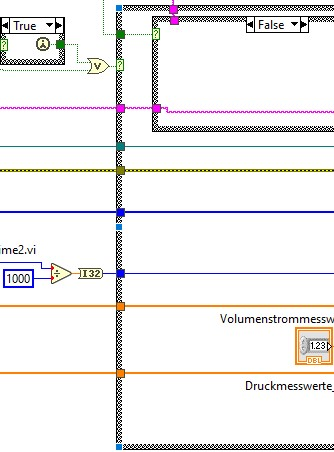
\includegraphics[width=0.3\textwidth]
            {Bilder/LabVIEW_serialport/datalogger_links_neu_false.jpg} %{Bilder/LabVIEW_serialport/}
        }
    \phantomcaption
    \vspace{1em}
    \ContinuedFloat
%\captionsetup{position=bottom}
    \subfloat[][Graph für zwei kontinuierliche Parameter \label{fig:Graphfürzwei}]{%
        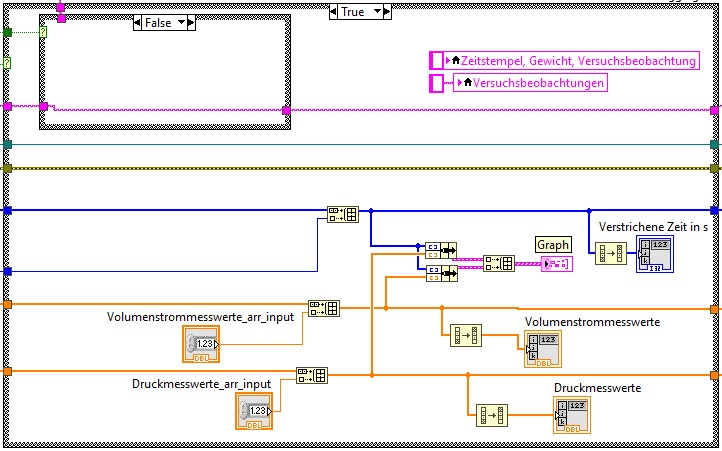
\includegraphics[width=0.9\textwidth]
        {Bilder/LabVIEW_serialport/datalogger_rechts_neu.jpg} %{Bilder/LabVIEW_serialport/}
    }
    \caption[Graph für zwei kontinuierliche Parameter]{Graph für zwei kontinuierliche Parameter}
    \label{}
\end{figure}



\paragraph{Achter Schritt: Diskrete Daten am Beispiel des Datalog Headers}

In der Abbildung \ref{fig:modularer_header} ist exemplarisch die erste Headerzeile (a) und die Methode (b), wie man diese mittels \textit{Concatenate} (17) verkettet abgebildet. Um eine schnelle und einfache Zusammenstellung der Headerkomponenten sowie die Übersichtlichkeit gewährleisten zu können, wird aus jedem Headereintrag ein Sub VI erstellt (siehe Abbildung \ref{fig:modularer_header} (b)). Der Datalogger Header ist somit einfach zu modifizieren.

%\newpage
%\begin{figure}[h] % Headerkonfiguration  standardheader Zeile und Zeitreihenheader
%     \subfloat[][Erste Header Zeile\label{fig:standard_header}]{%
%       \includegraphics[width=0.5\textwidth]
%       {Bilder/LabVIEW_serialport/standard_header.jpg}
%     }\hfill     
%    \subfloat[][Zeitreihen Überschrift\label{fig:header}]{%
%       \includegraphics[width=0.5\textwidth]
%      {Bilder/LabVIEW_serialport/header.jpg}
%     }\phantomcaption
%     %\caption[]{}
%%  \label{fig:simple_elapsed_time}
%   \end{figure}
%\begin{figure}[h] % Headerkonfiguration 2 Masse Dokumentenheader
%\ContinuedFloat
%\subfloat[][Masse Header Zeile\label{fig:vtp_masse}]{%
%       \includegraphics[width=0.5\textwidth]
%       {Bilder/LabVIEW_serialport/masse.jpg}
%     }\hfill     
%    \subfloat[][Verkettung der Headermodule\label{fig:dokumentenheader}]{%
%       \includegraphics[width=0.5\textwidth]
%      {Bilder/LabVIEW_serialport/Dokumentheaderverkettung.jpg}
%     }    
%\caption[Modulare Header Sub VI's]{Modulare Header Sub VI's}
%\label{fig:modularer_header}
%   \end{figure}

\begin{figure}[h] % Headerkonfiguration  standardheader Zeile und Zeitreihenheader
\centering
     \subfloat[][Erste Header Zeile\label{fig:standard_header}]{%
       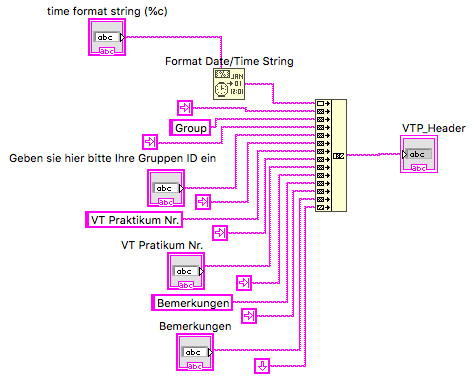
\includegraphics[width=0.49\textwidth]
       {Bilder/LabVIEW_serialport/standard_header.jpg}
     }%\hfill     
    \subfloat[][Verkettung der Headermodule\label{fig:dokumentenheader}]{%
       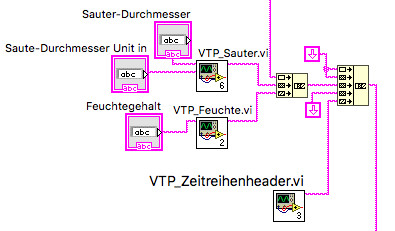
\includegraphics[width=0.49\textwidth]
      {Bilder/LabVIEW_serialport/Dokumentheaderverkettung.jpg}
     }    
\caption[Modulare Header Sub VI's]{Modulare Header Sub VI's}
\label{fig:modularer_header}
   \end{figure}

\paragraph{Neunter Schritt: Auslastungsoptimierung} Um die optimale Taktrate für das Programm empirisch zu ermitteln, kann man eine \,{\Menlo LED} (30) zwischen den Objekten \,{\Menlo Equal?} (26) und \,{\Menlo Not} (27) platzieren. Nun variiert man die Taktrate  der \textit{While Loop} des  \textit{Haupt VI's}, bis die \,{\Menlo LED} für die Optimierung blinkt, um Daten \textit{Just in Time} zu erhalten. Mit dem Objekt \,{\Menlo wait (ms)} (34) kann man eine Wartedauer vor jeder Iteration einstellen. Mit dem Objekt \,{\Menlo wait until next ms multiple} (35) kann man eine Taktzeit für einen Iteration einprogrammieren. Die Dauer der Pause, bzw. die Taktrate jeder Iteration sollte geringer sein als die Dauer die benötigt wird, um die Daten von dem seriellen Port auszulesen. Das Blinken signalisiert, dass der (Read Buffer) der Datenquelle nicht überfüllt (engl. \textit{buffer overflow}) wird. Damit ist gewährleistet, dass für das Ausführen des Programms \textbf{ nur soviel Rechenkapazität verwendet wird wie nötig, jedoch genug, damit keine Daten verloren gehen oder eine Totzeit entsteht!} Um die Taktrate rechnerisch zu ermitteln, benötigt man die zu erwartenden \,{\Menlo Bytes}, bzw. character pro Zeile. Die Baudrate (Bd) gibt an, wie viele \textbf{Zeichen} pro Sekunde versendet werden. In vielen fällen wird für 1\,\textbf{Zeichen},
\,1\,\,{\Menlo Bit} benötigt, daraus folgt, dass die Baudrate in diesen Fällen \,{\Menlo Bit} pro s bedeutet.\\

Um ein 7 \,{\Menlo Bit} encodiertes \,{\Menlo Byte} zu versenden, werden 3 weitere \,{\Menlo Bit} auf der Datenleitung versendet. In der Tabelle \ref{tab:678bit} sind die Konfigurationsmöglichkeiten bei der Nutzung von 6, 7 oder 8 \,{\Menlo Bit} Encodierung und RS-232.

\begin{table}[hpt!] %6, 7, 8 Bit Encodierung via RS-232
\caption{\,{\Menlo 6}, \,{\Menlo 7}, \,{\Menlo 8} \,{\Menlo Bit}-{\Menlo Encodierung} via RS-232}
\begin{center}
\begin{tabular}{|r|c|c|c|}
\cline{2-4}
\multicolumn{1}{c|}{} &	\,{\Menlo 6} \,{\Menlo Bit} 		& \,{\Menlo 7} \,{\Menlo Bit} 		& \,{\Menlo 8} \,{\Menlo Bit}\\
\hline
 \,{\Menlo Startbit} 				& \,{\Menlo 1}				 & \,{\Menlo 1} 			& \,{\Menlo 1}\\ \hline
 \,{\Menlo Symbol-/Characterbit} & \,{\Menlo 6} 			& \,{\Menlo 7} 			& \,{\Menlo 8}\\ \hline
 \,{\Menlo Paritätsbit} & \multicolumn{2}{c|}{\hspace{3pt} {\Menlo Odd/Even/Mark/Space} \hspace{3pt}} & \,{\Menlo none}  \\ \hline
\,{\Menlo Stoppbit}	& 	\,{\Menlo 2} &	\,{\Menlo 1}& \,{\Menlo 0}\\ \hline
\,{\Menlo Baudrate in Bd} & \multicolumn{3}{c|}{\hspace{3pt} {\Hypatia diverse Möglichkeiten} \hspace{3pt}}   \\ \hline
 \,{\Menlo Handshake} & \multicolumn{3}{c|}{\hspace{3pt} \,{\Menlo Software/Hardware} \hspace{3pt}}  \\ \hline
\end{tabular}
\end{center}
\label{tab:678bit}
\end{table}

Die Dauer zum empfangen einer \textbf{Zeile} (\,{\Menlo '+'} oder \,{\Menlo '-'} + floatnumber + potentiells \,{\Menlo 'g'}), die 7 oder 8 \,{\Menlo bit} ASCII encodiert ist und via RS-232 Schnittsttelle versendet wird , lässt sich wie folgt berechnen (Annahmen: Bd = 1200 $\frac{\,{\Menlo Byte}}{\mathrm{s}}$, 15 $\frac{\,{\Menlo Byte}}{\mathrm{Zeile}}$, 10 $\frac{\,{\Menlo Bit}}{\,{\Menlo Byte}}70
$). 


% Sendegeschwindigkeit pro Zeile
\begin{align} 
1	\mathrm{Bd} 	&=	1	\,	\mathrm{Zeichen/		\texttt{Bit} \,	pro \, Sekunde} \\
1	\, \,	\texttt{Byte}	&=	10	\, \,	\texttt{Bit} \\
15 \, \,	 \texttt{Byte} &= 1 \, \mathrm{Zeile} \\
 \frac{1}{1200}  \frac{\mathrm{s}}{\texttt{Bit}} \cdot
  10 \,\, \frac{\texttt{Bit}}{\texttt{Byte}} \cdot
   15 \,\,  \frac{\texttt{Byte}}{\mathrm{Zeile}} 	&=
    0,125 \, \mathrm{s \, pro \, Zeile} \\
    											&\equiv 125 \, \mathrm{ms \, pro \, Zeile}
\end{align}


\subsubsection{NI DAQmx Programmierung am Beispiel der Wirbelschichtanlage}

Neben Geräten, die einen integrierten analog digital Wandler haben, gibt es Sensoren, die lediglich das analoge Signal transmittieren. Folglich muss das analoge Signal in ein digitales Signal umgewandelt werden. Für den Fall das Sensoren keinen integrierten analog/digital Wandler besitzen, ist eine Messkarte zwischen Sensor und PC zu implementieren (siehe Abbildung \ref{fig:sensor_analog_schnittstelle}). \\

\begin{figure}[b!] %[htbp!] 
\centering
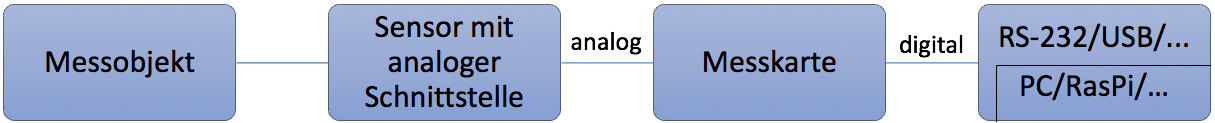
\includegraphics[width=1\textwidth]{Bilder/sensor_analoge_schnittstelle.jpg}
\vspace{0em}
 \caption[DAQ von Messeinrichtungen mit analoger Schnittstelle]{DAQ von Messeinrichtungen mit analoger Schnittstelle}\label{fig:sensor_analog_schnittstelle}
\end{figure}



\begin{figure}[b!] % 
% \captionsetup{position=top}
    \centering
        \subfloat[Druck- und Volumenstromsensor Initialisierung der Wirbelschicht][Druck- und Volumenstromsensor Initialisierung der Wirbelschicht \label{fig:daq_ini}]{%
            \hspace{0em}
            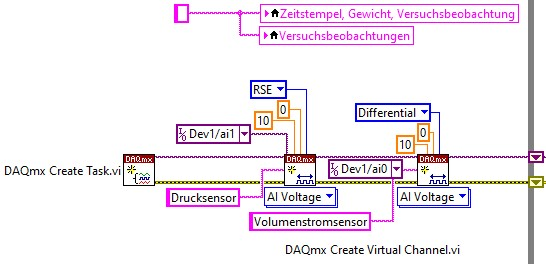
\includegraphics[width=0.7\textwidth]
            {Bilder/Wirbelschicht_Appfotos/Wirbelschicht_datai_DAQ_ini.jpg} %{Bilder/LabVIEW_serialport/}
        }
    \phantomcaption
    \vspace{1.5em}
    \ContinuedFloat
%\captionsetup{position=bottom}
    \subfloat[DAQ read sub vi options][DAQ read options \label{fig:DAQ_read_option}]{%
        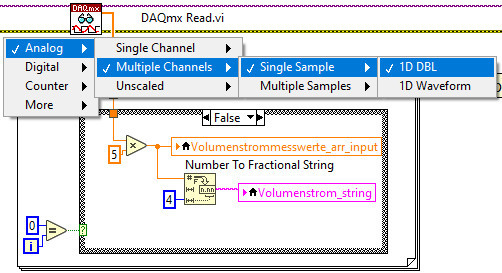
\includegraphics[width=0.7\textwidth]
        {Bilder/Wirbelschicht_Appfotos/Wirbelschicht_daq_read_option.jpg} %{Bilder/LabVIEW_serialport/}
    }
    \caption[DAQ Programmierung, Initialisierung und read.vi]{DAQ Programmierung, Initialisierung und read.vi}
    \label{fig:DAQ_Programmierung}
\end{figure}

Die NI Messkarte des Typs USB-6001 nennt sich in LabVIEW \textit{DAQmx}. Im folgenden Abschnitt wird die DAQ eines Volumenstromsensors und eines Druckssensors mittels USB-6001 Messkarte von National Instruments erläutert. In der Abbildung \ref{fig:daq_ini} ist die Initialisierungssequenz abgebildet, um analoge Signale von zwei Sensoren zu akquirieren. Es ist zu erkennen, das zwei Variablen (Zeitstempel,... ; Versuchsbeobachtungen), mittels lokaler Variable durch einem leeren String initialisiert werden.  Diese Form der Initialisierung hat eine Löschung der Werte aus der vorherigen Iteration zur Folge. Darunter ist die Initialisierung der DAQ Aufgabe (\textit{engl. task}), gefolgt von der Erstellung von zwei virtuellen Kanälen (\textit{engl. channel}) zu erkennen. Die Reihenfolge wurde zufällig gewählt. Es ist zu erkennen, dass der erste \,{\Menlo channel} den Drucksensor abfragt. Für den Drucksensor ist der Modus Operandi (Betriebsmodus) single ended ({\Menlo RSE}) auszuwählen. Die minimalen und maximalen Signal- bzw. Spannungswerte entsprechen 0~und~10~V. Der Drucksensors ist an Slot {\Menlo ai1} angeklemmt. Das DAQmx Gerät hat im System die Kennung {\Menlo Dev1} erhalten, daraus folgt das der Slot {\Menlo \,Dev1/ai1} auszuwählen ist. Für den Volumenstromsensor ist analog vorzugehen. Gemäß der elektrotechnischen Verschaltung (siehe Abbildung \ref{fig:wirbelelektrotechnik} im Abschnitt \ref{sec:schaltung}) ist das Signal des Volumenstromsensors nach dem Strom-/Spannugnswandler differenziel (double ended), daher ist als Modus \,{\Menlo Differentiall} auszuwählen.  Die Signalspanne ist analog des Drucksensors von 0~bis~10~V. Der Draht mit den Messignalen und der Errordraht betreten die While-Loop via \,{\Menlo Shift Register}. Das Auslesen wird mit dem {\Menlo DAQmx~Read.vi}, mit den Optionen gemäß \ref{fig:DAQ_read_option} durchgeführt.\\



An der Stelle muss die serielle Abfrage Programmiert werden. In der Abbildung \ref{fig:Druck_DAQ} ist zu erkennen, dass der \textit{\textbf{for loop} tunnel} (ist am \textcolor{blue}{{\Menlo N}} zu erkennen) ein weißer Kasten mit orangen Klammern ist. Das bedeutet, dass die \textbf{\textit{for loop}} betretenden Werte indexiert sind. Während \textbf{einer \textit{while loop} Iteration} erfolgen \textbf{zwei \textit{for loop} Iterationen}. Zur Erinnerung wird an dieser Stelle noch mal erwähnt, dass LabVIEW alles (Arrays, Schleifen etc.) mit dem Index null initiiert. Pro \textit{\textbf{while loop}} Iteration werden die Werte, die in die \textbf{\textit{for loop}} eintreten  also immer mit 0 und 1 indexiert. Der case structure selector muss mit dem \,{\Menlo equal?} Vergleichsoperator abfragen, ob der Wert 0 oder 1 ist. Das Signal des Drucksensors hat den Index 0, da es der erste channel ist, der initialisiert wird (vgl. Abbildung \ref{fig:daq_ini}). An dieser Stelle ist nun ein Gleichungssystem zu lösen. Der Sensor hat eine Messspanne von -1~bis~1~bar. Das elektrische Signal geht von 0~bis~10~V. Gemäß Abschnitt \ref{sec:quader} ist die Approximation durch eine Gerade hinreichend. Daraus folgt, dass für den Fall, dass die Spannung am DAQ Gleich 0 ist folgende Gleichung:

\begin{align}
p&=a \cdot x+b \\
-1~\mathrm{bar} &= a \cdot 0~\mathrm{V}+b \\
-1~\mathrm{bar} &=b \label{eq:druck_pt1}
\end{align}

Für den Fall, dass die Messkarte 10~$\mathrm{V}$ anzeigt gilt in Kombination mit Gleichung \ref{eq:druck_pt1}

\begin{align}
1~\mathrm{bar} &=a \cdot 10~\mathrm{V} -1~\mathrm{bar} \\[0.5em]
a &= \frac{1~\mathrm{bar}+1~\mathrm{bar}}{10~\mathrm{V}} \\[0.5em]
a &= \frac{2~\mathrm{bar}}{10~\mathrm{V}} \\[0.5em]
p &= 0,2~\frac{\mathrm{bar}} {\mathrm{V}}-1~bar
\end{align}

Da ein linearer Zusammenhang besteht und der Druck relativ zur Atmosphäre angegeben wir kann der offset durch die Addition des atmosphärischen Drucks $1~\mathrm{bar}$ eliminiert werden. Der Multiplikationsfaktor 0,2~$\frac{\mathrm{bar}}{\mathrm{V}}$ ist somit der gesuchte Wert für die Signalumrechnung.\\

In der Abbildung \ref{fig:analog-digitaldrucksensor} ist der Vergleich der Analog- und Digitaldruckmessung als Funktion des analog gemessenen Durchfluss zu erkennen. Des Weiteren wurde von beiden Messwertreihen eine lineare Approximationsfunktion erstellt. Der Drucksensor hat zum Zeitpunkt dieser Messung in der LabVIEW Applikation (als Konstante) \textbf{zwei} signifikante Stellen. Eine Wiederholung dieser Messung wird empfohlen, daher wird auf eine Anzeige der Approximationsfunktion zur Berechnung der Geraden verzichtet. In der LabVIEW Applikation ist für den Drucksensor die Anzahl der signifikanten Nachkommastellen auf \textbf{vier} korrigiert worden (siehe Abbildung \ref{fig:DAQ_Programmierung}).\\

\begin{figure}[h!] %[htbp!] 
\centering
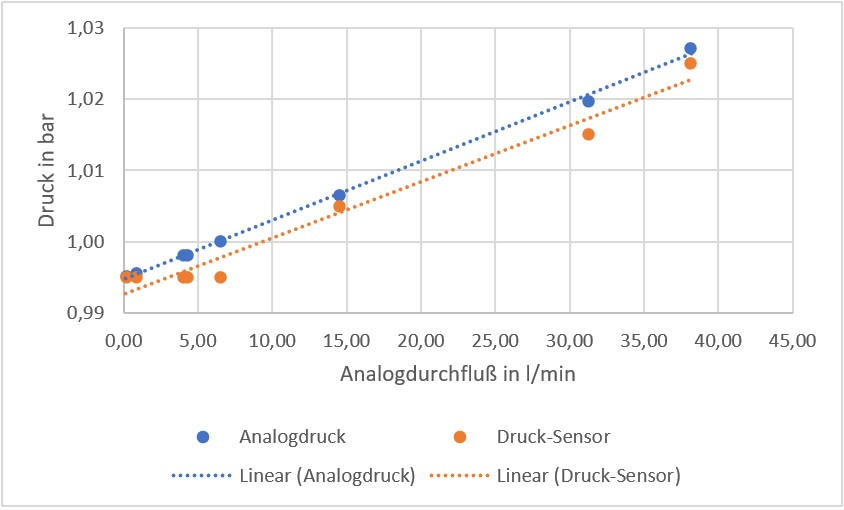
\includegraphics[width=0.8\textwidth]{Bilder/analog-digitaldrucksensor.jpg}
\vspace{0em}
 \caption[Analog-, Digitaldruckmessung als Funktion der analogen Volumenstrommesswerte]
{Analog-, Digitaldruckmessung als Funktion der analogen Volumenstrommesswerte}\label{fig:analog-digitaldrucksensor}
\end{figure}

In einem thermischen Massendurchflusssensor ist eine Wheatstone`sche Brückenschaltung als elektrotechnische Komponente verbaut. Das elektrische Ausgangssignal des Sensors ist demnach ebenfalls linear. Für den Volumenstromsensor ist folglich analog vorzugehen. Der Parameter $a$ des Volumenstromsensor ist somit $5~\frac{\mathrm{l}/\mathrm{min}}{\mathrm{V}}$, mit $b=0~\frac{\mathrm{l}}{\mathrm{min}}$.\\

In der Abbildung \ref{fig:volumenstrom_messung} ist eine Volumenstrommessung, analog sowie digital, sowie der Betrag der absoluten Differenz beider Messwertreihen als Funktion der Manometerdruckdifferenz in mm abgebildet. Bei beiden Messwertreihen ist ein linearer Zusammenhang zu erkennen. In Folge dessen wurden lineare Approximationsfunktionen erstellt. Des Weiteren ist zu erkennen, dass beide Messwertreihen divergieren. Die größte Abweichung hat einen Betrag von 6,7~$\frac{\mathrm{l}}{\mathrm{min}}$ Da der \glqq Wahre\grqq{} Wert unbekannt ist wird keine relative Abweichung sowie Standardabweichung ermittelt.\\ 



\begin{figure}[h!] %[htbp!] 
\centering
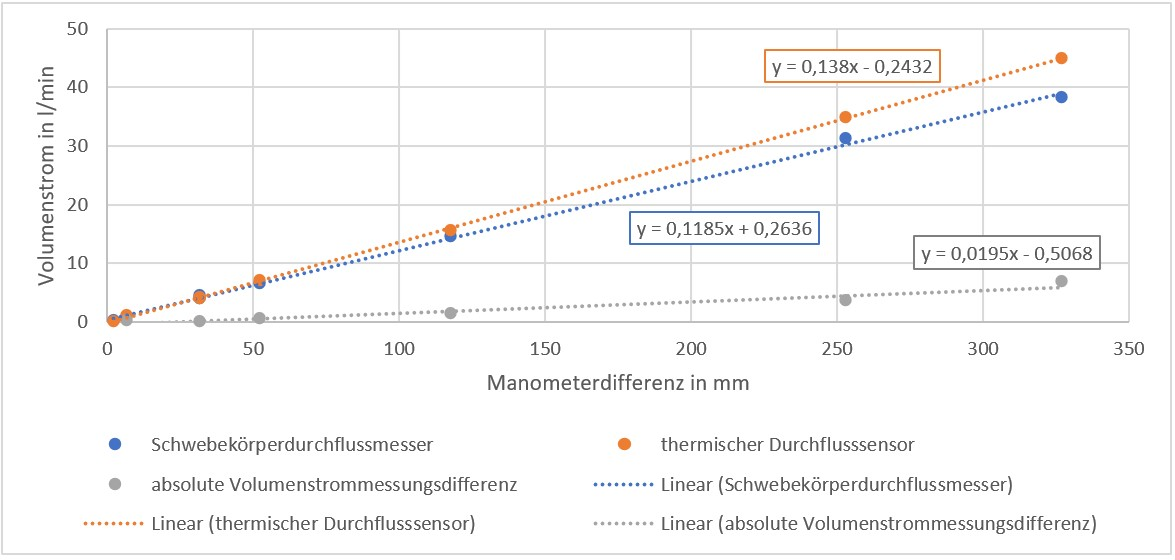
\includegraphics[width=1\textwidth]{Bilder/Volumenstrommessungsverleich.jpg}
\vspace{0em}
 \caption[Analog-/Digitalvolumenstrommessung sowie absolute Abweichung in l/min, als Funktion der Manometerdifferenz in mm]
{Analog-/Digitalvolumenstrommessung sowie absolute Abweichung in l/min, als Funktion der Manometerdifferenz in mm}\label{fig:volumenstrom_messung}
\end{figure}

\begin{figure}[h!] % 
% \captionsetup{position=top}
    \centering    
    \subfloat[Druck DAQ][Druck DAQ \label{fig:Druck_DAQ}]{%
        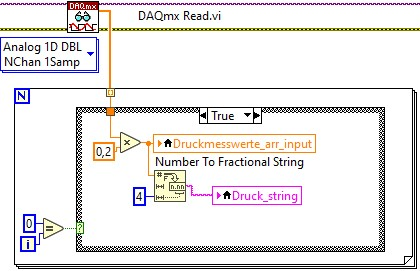
\includegraphics[width=0.6\textwidth]
        {Bilder/Wirbelschicht_Appfotos/druck_daq.jpg} %{Bilder/LabVIEW_serialport/}
    }
     \hspace{0.06em}
         \subfloat[][Clear Task \label{fig:clear_task}]{%
            \hspace{0em}
            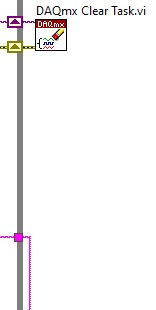
\includegraphics[width=0.206\textwidth]
            {Bilder/Wirbelschicht_Appfotos/daq_endsequenz.jpg} %{Bilder/LabVIEW_serialport/}
        }
    \phantomcaption
    \vspace{1em}
    \ContinuedFloat
%\captionsetup{position=bottom}
     \subfloat[Volumenstrom DAQ][Volumenstrom DAQ \label{fig:Volumenstrom_DAQ}]{%
            \hspace{0em}
            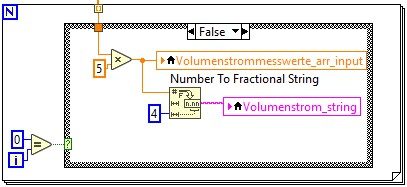
\includegraphics[width=0.6\textwidth]
            {Bilder/Wirbelschicht_Appfotos/Volumenstrom_daq.jpg} %{Bilder/LabVIEW_serialport/}
        }
       
    \caption[DAQ und interpretation beider kontinuierlichen Paramter, Druck und Volumenstrom]
    {DAQ und interpretation beider kontinuierlichen Paramter, Druck und Volumenstrom}
    \label{fig:daq_p_v}
\end{figure}



Bei der Beendigung des Programms musst der DAQmx task terminiert werden, dafür ist das {\Menlo DAQmx Clear Task.vi} außerhalb der \textit{while loop} zu platzieren und mit dem Signal sowie error {\Menlo schift \mbox{register}} zu verbinden  (siehe Abbildung \ref{fig:clear_task}).


\paragraph{Haupt Programm Dataloggerintialisierung am Beispiel der Filterkuchenversuchsanlage} 
Im Verlauf des Projekts ist der Wunsch geäußert worden, dass die generierten Protokolle unveränderlich (Schreibschutz) sein sollen. Der Dateidialog (siehe Abbildung \ref{fig:Dateidialog} im Anhang) wird vor der Schreibschutzabfrage platziert (siehe Abbildung \ref{fig:schreibschutz_dialog}) und, im Falle einer versuchten Öffnung einer Datei mit Schreibschutzes, in der \,{\Menlo case structure} \, (\textcolor{OliveGreen}{{\Menlo No Error}}) entfernt. Im \,\textcolor{red}{{\Menlo Error}} {\Menlo case} werden die Tunnel beider Seiten verbunden (siehe Abbildung \ref{fig:schreibschutz_dialog}). Auf weitere Erläuterungen wird im Rahmen dieser Arbeit verzichtet
\label{sec:Pfad}

\begin{figure}[h!] %[htbp!] 
\centering
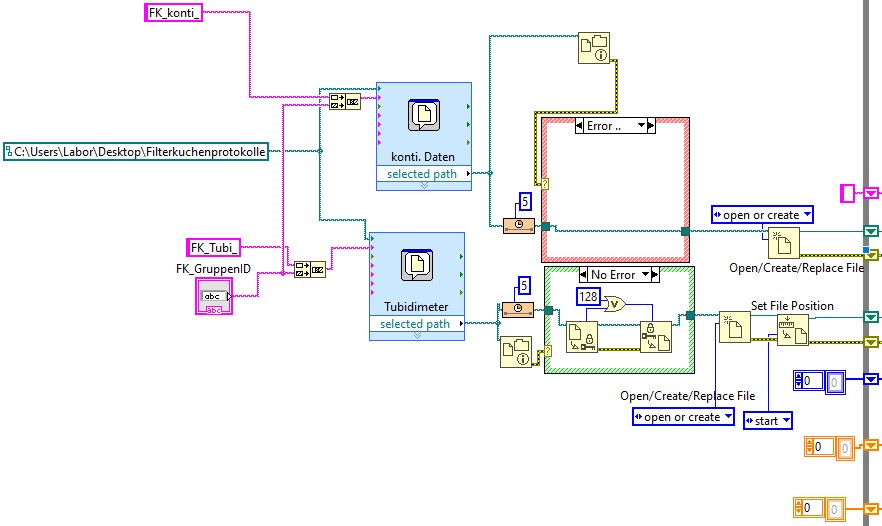
\includegraphics[width=0.8\textwidth]{Bilder/LabVIEW_serialport/Haupt_VI_unten_links_3.jpg}
\vspace{0em}
 \caption[Dataloggerinitialiserung]
{Dataloggerinitialiserung}\label{fig:schreibschutz_dialog}
\end{figure}


\paragraph{Haupt Programm Dataloggerheader am Beispiel der Filterkuchenversuchsanlage} 

An der Abbildung \ref{fig:filterkuchenheader} lässt sich erahnen, dass die Erstellung diskreter Daten in LabVIEW eine tiefgreifende Verschachtlungen mittels eigens erstellter Sub VI`s benötigt. Auf eine Erläuterungen wird im Rahmen dieser Arbeit verzichtet. Es ist zu erkennen, dass der verkettete String aus der \,{\Menlo while loop} geführt wird. \\

Im Verlauf des Projekts wurde der Wunsch geäußert eine weitere Datei, mit sogenannten Tubidimeter Daten, generieren zu lassen. Analog des Headers ist eine verschachtelte Programmierung der Tubidimeter Eingaben erfolgt. Auf eine Erläuterungen wird im Rahmen dieser Arbeit verzichtet. Diese Daten werden während der Versuchsdurchführung, nach der Beendigung (\,{\Menlo Stop}-Button im Frontpanel siehe Abbildung \ref{fig:FilterkuchenVersuchseingaben}) eines Messungsdurchlaufs eingefügt. Es werden laut Praktikumsanweisung pro Versuchstag hintereinander drei Messungen durchgeführt. Das Schreiben, in die Datei mit den kontinuierlichen Daten und in die Datei mit den Tubidimeter Daten, muss sich an der Stelle unterscheiden. Für die Tubidimeterdatei muss die gesamte Datei Überschrieben werden und nicht wie im Fall der kontinuierlichen Datei am Ende angehängt. \,{\Menlo Set File Position.vi} erhält an dieser Stelle die Konstante \,{\Menlo start} (siehe Abbildung \ref{fig:schreibschutz_dialog}).

\begin{figure}[h!] %[htbp!] 
\centering
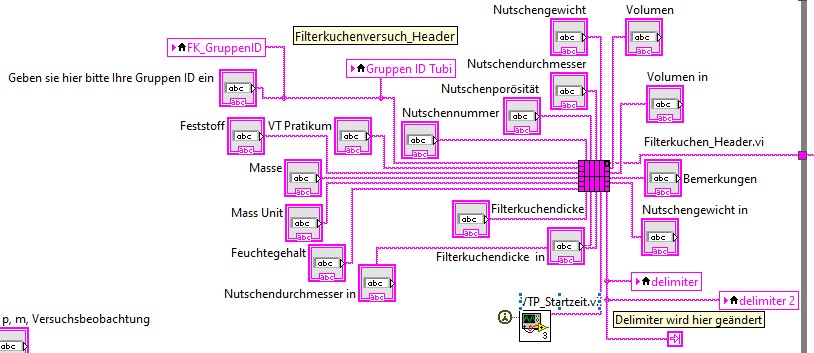
\includegraphics[width=0.9\textwidth]{Bilder/LabVIEW_serialport/Filterkuchenheader.jpg}
\vspace{0em}
 \caption[Filterkuchenheader]
{Filterkuchenheader}\label{fig:filterkuchenheader}
\end{figure}

\paragraph{Haupt Programm Endsequenz}

Wird das Hauptprogramm via \,{\Menlo Stop}-Button beendet, dann erfolgt die Endsequenz gemäß Abbildung \ref{fig:endsequenz}. Die Daten werden an dieser Stelle in die geöffnete bzw. erstellte Datei geschrieben, diese Datei geschlossen und mit einem Schreibschutz versehen.  

\begin{figure}[h!] %[htbp!] 
 \centering
 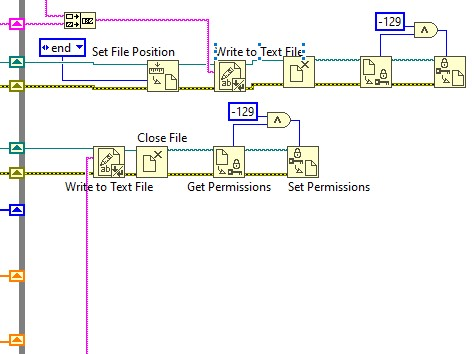
\includegraphics[width=0.6\textwidth]{Bilder/LabVIEW_serialport/endsequenz.jpg}
 \vspace{0em}
  \caption[Endsequenz des Hauptprogramms]
 {Endsequenz des Hauptprogramms}\label{fig:endsequenz}
 \end{figure} 
\pagebreak

\subsection{Verwendung beider Programme}
\label{sec:Haupt_VI_Nutzung}

Damit die Kommentarfunktion wie gewünscht funktioniert, ist vor der Verwendung des Programms in den LabVIEW Einstellungen unter Environment \,{\Menlo  End Text entry with Enter key} einzustellen (siehe Abbildung \ref{endtextentry}). Ist diese Option nicht eingestellt, muss nach jeder Betätigung der \,{\Menlo Enter}-Taste, die Eingabe ein weiteres mal mittels eines Mausklicks auf einen schwarzen Haken, der neben dem VI Ausführen Pfeil (oben links im Front Panel) erscheint, quittiert werden.

\bild{0.7}
{LabVIEW_serialport/endtextentry.png}
{0em}
{Einstellung \glqq End text entry with Enter key\grqq{}}
{Einstellung \glqq End text entry with Enter key\grqq{}}
{endtextentry}

Es wurde eine \,{\Menlo Tab Control} verwendet, um verschiedene Registerfenster zu generieren, siehe folgende Liste:

\begin{itemize} % Haupt VI Reiter
\singlespacing
\item Versuchseingaben
\item Während der Messung
\item Tubidimeter
\item \textcolor{black!50}{Konfiguration}
\item \textcolor{black!50}{Debugging}
\end{itemize}

Wie der Liste (\textcolor{black!50}{Markierung}) und der Abbildung \ref{fig:FilterkuchenVersuchseingaben} zu entnehmen ist, sind die Tabs \textcolor{black!50}{Konfiguration} und \textcolor{black!50}{Debugging} nicht sichtbar. Zum erreichen dieser Tabs ist das Frontpanel mit einem Passwort zu entsperren (z.B. durch die Betätigung von \,{\Menlo Strg+E}) und gemäß Abbildung \ref{fig:Filterkuchen_go_to_debugging} im Anhang fortzufahren. \\

In der Abbildung \ref{fig:FilterkuchenVersuchseingaben} ist das Frontpanel für den Filterkuchenversuchstand abgebildet. Oben links im Bild ist das Programmstarticon $\Rightarrow$ zu erkennen. Für den Wirbelschichtversuchsstand sieht das Frontpanel identisch aus.\\

\begin{figure}[h!] %[htbp!] 
\centering
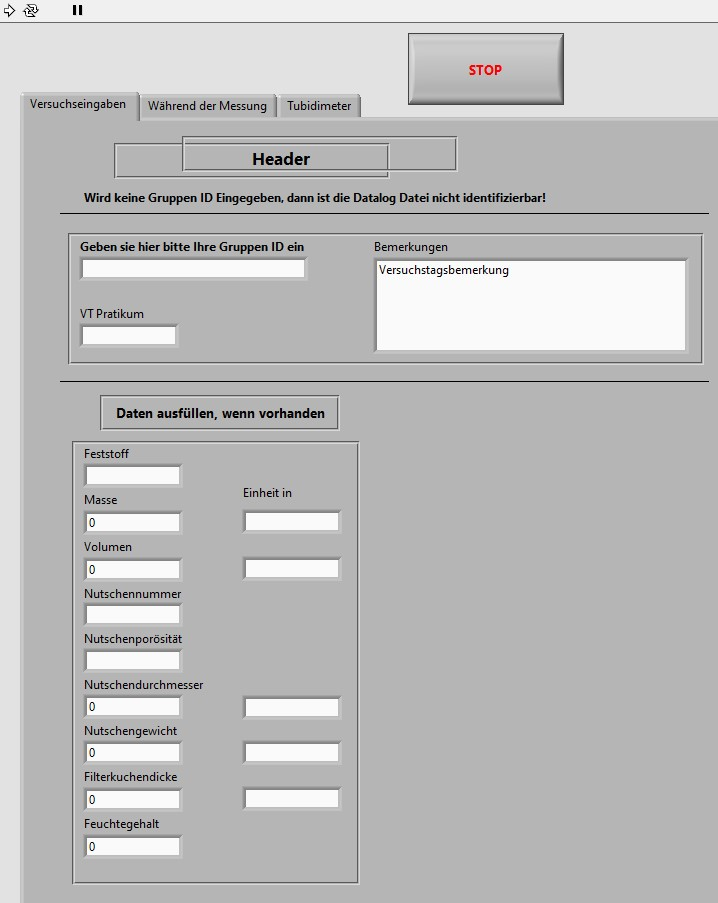
\includegraphics[width=0.8\textwidth]{Bilder/Filterkuchen_Appfotos/FK_Versuchseingaben.jpg}
\vspace{0em}
 \caption[Filterkuchen Frontpanel: Versuchseingaben]
{Filterkuchen Frontpanel: Versuchseingaben}\label{fig:FilterkuchenVersuchseingaben}
\end{figure}

Die Frontpanel Tabs für die kontinuierlichen Messungen sehen für beide Versuchsstände identisch aus (siehe Abbildung  \ref{fig:messung}). Unter dem Plotter ist links ein Eingabefeld für Versuchsbeobachten zu erkennen. Die Eingaben werden dem Zeitstempel, zum Zeitpunkt der \,{\Menlo Enter}betätigung, angehängt. Rechts von dem Eingabefeld für die Versuchsbeobachtungen sind die Arrays abgebildet, die oben den aktuellsten Messwert anzeigen. Das Schreiben der kontinuierlichen Daten (in einen String) erfolgt erst nach Betätigung des Buttons \,{\Menlo Start Datalogging in Tabgetrennt.txt Datei}. Die Endsequenz, in der die Daten der kontinuierlichen Messung sowie die der Tubidimetereingaben (siehe Abbildung \ref{fig:tubidimetereingaben}), in die geöffnete oder generierten Datei geschrieben werden, erfolgt nach dem Betätigen des \,{\Menlo Stop}-Buttons (siehe Abbildung \ref{fig:FilterkuchenVersuchseingaben}). 

\begin{figure}[h!] %[htbp!] 
\centering
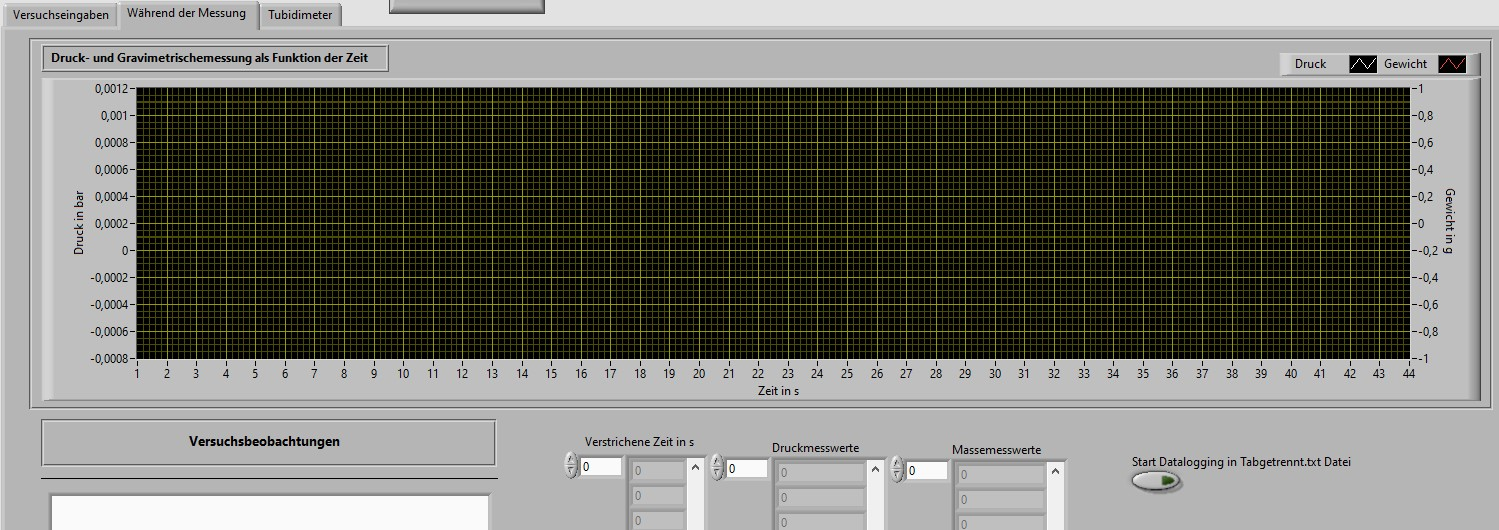
\includegraphics[width=1\textwidth]{Bilder/Filterkuchen_Appfotos/Filterkuchen_diagramm.jpg}
\vspace{0em}
 \caption[Filterkuchen Frontpanel: Tab der kontinuierlichen Messung am Beispiel der Filterkuchenapplikation]
{Tab der kontinuierlichen Messung am Beispiel der Filterkuchenapplikation}\label{fig:messung}
\end{figure}

\begin{figure}[h!] %[htbp!] 
\centering
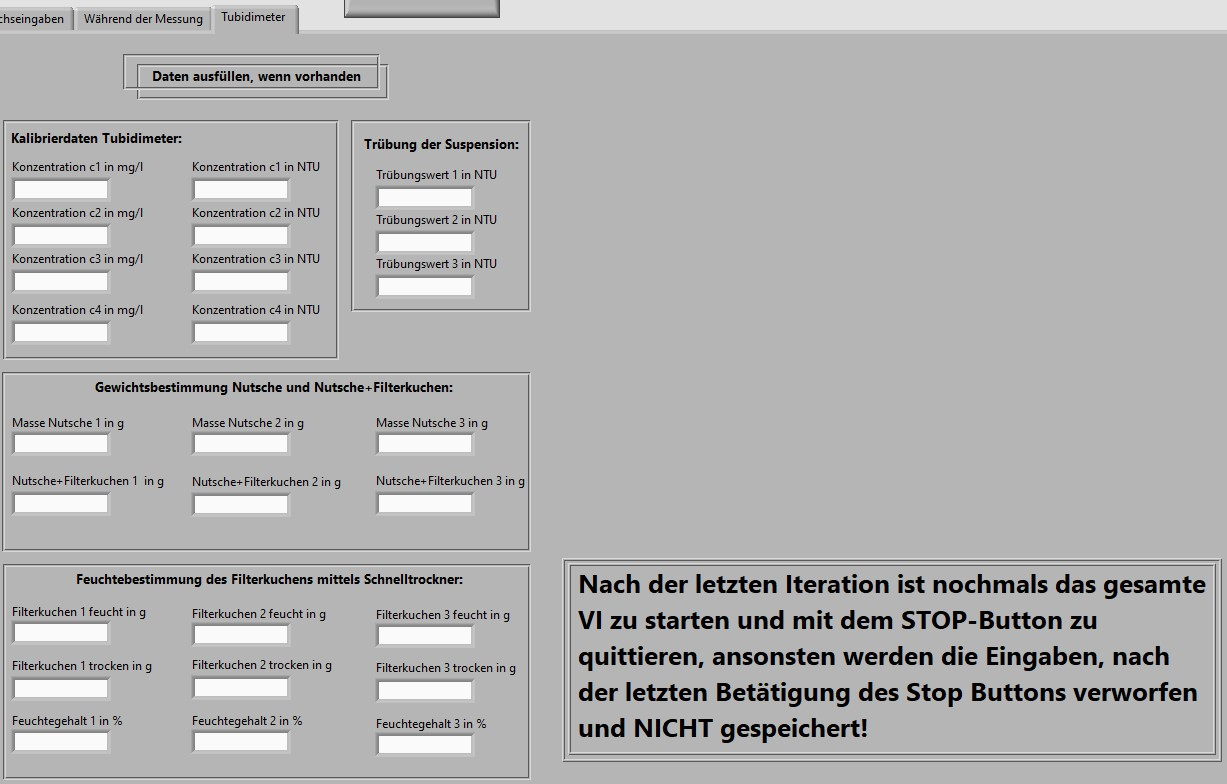
\includegraphics[width=1.07\textwidth]{Bilder/Filterkuchen_Appfotos/Tubidimeter_FP_Eingaben.jpg}
\vspace{0em}
 \caption[Filterkuchen Frontpanel: Tab der Tubidimetereingaben]
{Filterkuchen Frontpanel: Tab der Tubidimetereingaben}\label{fig:tubidimetereingaben}
\end{figure}



In der Abbildung \ref{fig:funktionstest} ist ein Datalog eines Wirbelschichtestdurchlaufs zu erkennen. Diese \,{\Menlo .txt} Datei wurde in Excel Importiert. Es ist zu erkennen, dass diese Messwerte vier signifikante Stellen aufweisen. Es kann vorkommen, dass die automatische Datenimportfunktion das Spaltentrennzeichen nicht erkennt, dann ist gemäß Micosofts Problembehungshinweis fortzufahren (siehe Teilausschnitt in Abbildung \ref{fig:legacy}). Im Falle der Tubidimeterdatei ist dies der Fall gewesen, daher wird der Import nicht automatisch eingefärbt (siehe Abbildung \ref{fig:tubidimeter_import}). Des Weiteren ist zu erkennen, dass die Eingaben keine Restriktionen enthalten (int8, 16, 32, 64; float8, ...; die Ziffer steht für die Bytelänge). Alle Eingaben sind \,{\Menlo Strings}, dass bedeutet, es ist im Textformat. Bei der Weiterverarbeitung ist eine Umwandlung in ein int oder float zu erfolgen (in Excel\,{\Menlo  Zelle formatieren..}).


\begin{figure}[h!] % 
% \captionsetup{position=top}
    \centering
      \vspace{-1em}
        \subfloat[Datalogimport der kontinuierlichen Daten in Excel, am Beispiel der Wirbelschicht Daten]
        [Datalogimport der kontinuierlichen Daten in Excel, am Beispiel der Wirbelschicht Daten \label{fig:funktionstest}]{%
            \hspace{0em}
            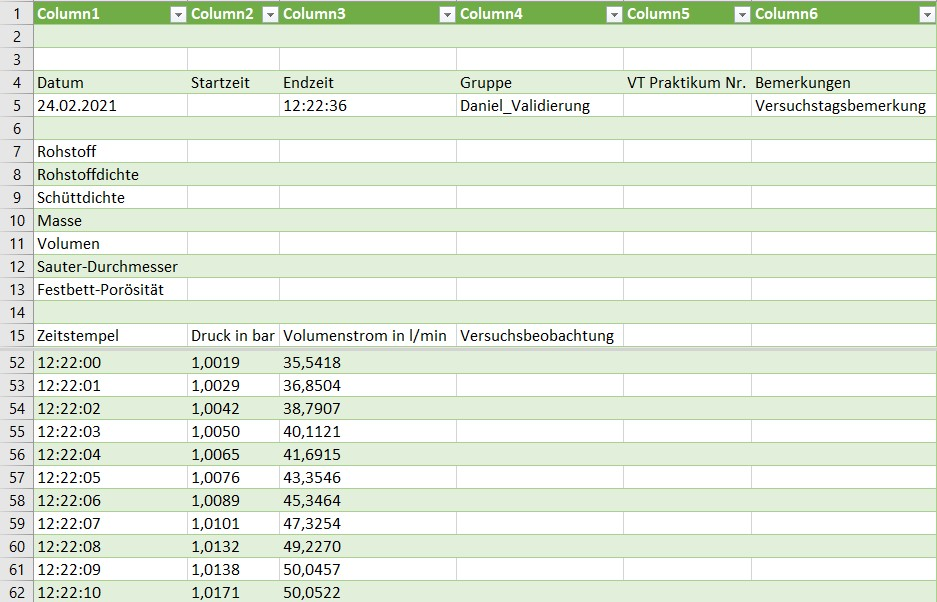
\includegraphics[width=0.7\textwidth]
            {Bilder/Wirbelschicht_Appfotos/Wirbelschicht_Versuchseingaben_datalog_klein.jpg} %{Bilder/LabVIEW_serialport/}
        }
    \phantomcaption
    \vspace{0.7em}
    \ContinuedFloat
%\captionsetup{position=bottom}
    \subfloat[Legacy Import, gemäß Microsoft][Legacy Import, gemäß Microsoft \label{fig:legacy}]{%
        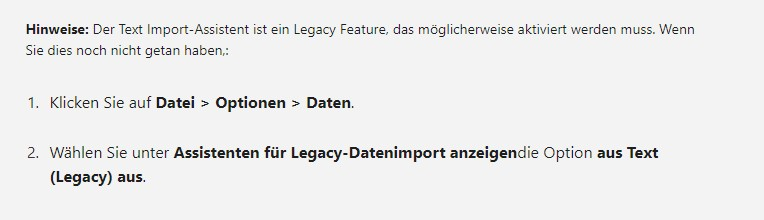
\includegraphics[width=0.7\textwidth]
        {Bilder/ms_legacy.jpg} %{Bilder/LabVIEW_serialport/}
    }
     \phantomcaption
    \vspace{0.7em}
    \ContinuedFloat
%\captionsetup{position=bottom}
    \subfloat[Tubidimeter Datalogimport in Excel][Tubidimeter Datalogimport in Excel \label{fig:tubidimeter_import}]{%
        \includegraphics[width=0.7\textwidth]
        {Bilder/Filterkuchen_Appfotos/tubidimeter.jpg} %{Bilder/LabVIEW_serialport/}
    }
    \caption[Datalogs und Excel troubleshooting]{Datalogs und Excel troubleshooting}
    \label{}
\end{figure}


%\begin{figure}[h!] %[htbp!] 
%\centering
%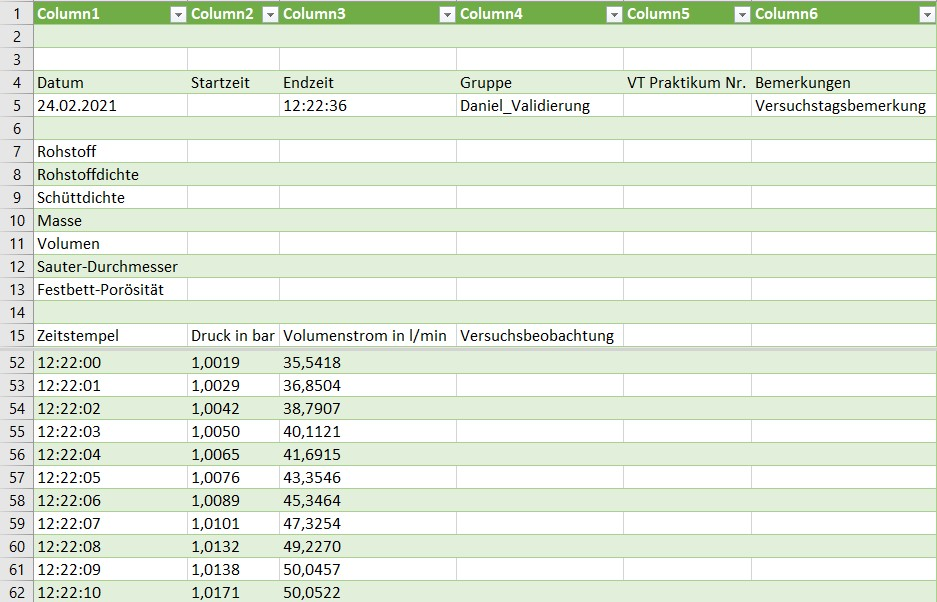
\includegraphics[width=0.7\textwidth]{Bilder/Wirbelschicht_Appfotos/Wirbelschicht_Versuchseingaben_datalog_klein.jpg}
%\vspace{0em}
% \caption[Datalogimport der kontinuierlichen Daten in Excel, am Beispiel der Wirbelschicht Daten]
%{Datalogimport der kontinuierlichen Daten in Excel, am Beispiel der Wirbelschicht Daten}\label{fig:funktionstest}
%\end{figure}

%\begin{figure}[h!] %[htbp!] 
%\centering
%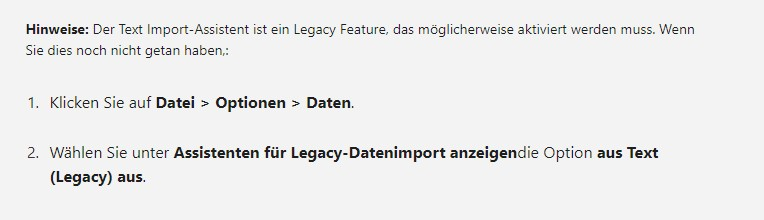
\includegraphics[width=0.8\textwidth]{Bilder/ms_legacy.jpg}
%\vspace{0em}
% \caption[Legacy Import, gemäß Microsoft]
%{Legacy Import, gemäß\cite{Windows2021}}\label{fig:legacy}
%\end{figure}

%\begin{figure}[h!] %[htbp!] 
%\centering
%\includegraphics[width=0.6\textwidth]{Bilder/Filterkuchen_Appfotos/tubidimeter.jpg}
%\vspace{0em}
% \caption[Tubidimeter Datalogimport in Excel]
%{Tubidimeter Datalogimport in Excel}\label{fig:tubidimeter_import}
%\end{figure}



\FloatBarrier

\subsubsection{Fazit}

Die implementation eines Cloudservice (HAW Cloud) ist im Verlauf des Projekts nicht erfolgt. Die HAW Richtlinien scheinen es \textbf{derzeit} nicht zu gestatten, dass Kennungen an nicht humane Entitäten bzw. nicht natürliche Personen vergeben werden. Nicht humane Entitäten könnten die folgenden sein:
 
\begin{itemize}
\item Geräte
\begin{itemize}
\item HMI's 
\item Sensoren
\end{itemize} 
\item Aggregate
\item Maschinen
\end{itemize}

Die Idee, dass jeder Laboraccount eine eigene Kennung erhält, wodurch die Laborgeräte wie HMI's ein Cloudverzeichnis auf der HAW Cloud erhalten würden, ist derzeit nicht realisierbar. Die Idee, dass nicht humane Entitäten eine Kennung erhalten können, sollte in höheren Instanzen der HAW diskutiert werden, damit zukünftige Cloudlösungen HAW global realisiert werden können. Die Hochschule sollte das Ziel haben die Privatwirtschaft abzubilden. Das nicht humane Entitäten ein eigenes Kommunikationbsnetzwerk erhalten ist bereits Stand der Technik (siehe Abschnitt \ref{sec:bluetooth}). \\

Es ist anzumerken, dass die \,{\Menlo Controls} für die diskreten Eingaben keine Eingaberestriktionen besitzen und alles im Textformat gespeichert wird.

\pagebreak